
\chapter{Control of Multi-Rotor Aircraft}\label{chapter:control}

\textit{Now that a sufficiently accurate mathematical model of the hexacopter has been developed, the control problem is able to be approached. Within this chapter two control systems will be developed with the aim of controlling the aircraft position and attitude. Simulations will then be performed in Simulink to verify the effectiveness of each control system. For the purposes of these simulations it will be assumed that the vehicle's position and attitude (x, y, z, $\phi$, $\theta$, $\psi$) can be accurately measured at any given time.} 

\section{Pseudo-inverse of Motor Speed Matrix}
The control systems in this chapter will be based upon the effective inputs of the plant i.e. $\tau_{\phi}$, $\tau_{\theta}$, $\tau_{\psi}$, $F_{T}$. Therefore, it will be necessary to implement an inverse of the matrix in \eqref{eqn:propSpeeds1} in order to obtain the desired input motor speeds. This matrix is not square and is therefore not invertible. However, for a matrix A with linearly independent rows, the Penrose-Moore pseudo-inverse ($A^{+}$) is able to be computed such  that: 
\[A^{+}= A^{T}(AA^{T})^{-1}\]
In this case, this is a right inverse which will satisfy \(AA^{+}=I\) where I is an identity matrix. The pseudo-inverse matrix is shown in \eqref{eqn:propSpeeds2} and will be used to reverse the relationship between the effective inputs and the propeller speeds.
\begin{equation}\label{eqn:propSpeeds2}
\begin{bmatrix}
\Omega^{2}_{1}\\
\Omega^{2}_{2}\\
\Omega^{2}_{3}\\
\Omega^{2}_{4}\\
\Omega^{2}_{5}\\
\Omega^{2}_{6}\\
\end{bmatrix}
=
\begin{bmatrix}
-\frac{1}{6C_{T}d} & \frac{\sqrt{3}}{(6C_{T}d)} &  \frac{1}{6K_{psi}} & \frac{1}{6C_{T}}\\
-\frac{1}{3C_{T}d} & 0 & -\frac{1}{6K_{psi}} & \frac{1}{6C_{T}}\\
-\frac{1}{6C_{T}d} & -\frac{\sqrt{3}}{(6C_{T}d)} & \frac{1}{6K_{psi}} & \frac{1}{6C_{T}}\\
 \frac{1}{6C_{T}d} & -\frac{\sqrt{3}}{(6C_{T}d)} & -\frac{1}{6K_{psi}} & \frac{1}{6C_{T}}\\
 \frac{1}{3C_{T}d} & 0 & \frac{1}{6K_{psi}} & \frac{1}{6C_{T}}\\
 \frac{1}{6C_{T}d} &  \frac{\sqrt{3}}{(6C_{T}d)} & -\frac{1}{6K_{psi}} & \frac{1}{6C_{T}}
\end{bmatrix}
\begin{bmatrix}
\tau_{\phi}\\
\tau_{\theta}\\
\tau_{\psi}\\
F_{T}\\
\end{bmatrix}
\end{equation}

This relationship is simulated as a subsystem in the Simulink model and is shown in Appendix \ref{section:Simu_Motor}.

\section{PID Control}\label{section:PIDControl}
Initially, a control strategy for the hexacopter will be developed based upon Proportional Integral Derivative (PID) control. The basic concept of PID control is outlined in Section \ref{section:PIDBackground}. This controller will be designed with the aim of stabilising the vehicle around a hovering point and this allows the model to be simplified.
\subsection{Simplified Model}\label{section:SimpleModel}
For the purposes of this controller, the vehicle will be assumed to be hovering, which implies the roll and pitch angles ($\phi$ $\theta$) will only have small variations from the origin. These assumptions will be used in developing the controller, however the controller will be verified by simulation on the full nonlinear model. Likewise, we will assume the yaw angle ($\psi$) is held close to the origin. This allows the small angle approximation to be applied to the model defined in Section \ref{section:ModelDynamics}. Applying this assumption to \eqref{eqn:state1} gives \eqref{eqn:simpleState1}.

\begin{equation}\label{eqn:simpleState1}
\begin{split}
\begin{bmatrix}
\dot{\phi}\\ \dot{\theta} \\ \dot{\psi}
\end{bmatrix} 
&=
\begin{bmatrix}
1 & 0 & 0\\
0 & 1 & 0\\
0 & 0 & 1
\end{bmatrix}
\begin{bmatrix}
p\\q\\r
\end{bmatrix} \\
\begin{bmatrix}
\dot{\phi}\\ \dot{\theta} \\ \dot{\psi}
\end{bmatrix} 
&=
\begin{bmatrix}
p\\q\\r
\end{bmatrix}
\end{split}
\end{equation} 




Likewise, it will be assumed that p, q and r are significantly small when compared with the input torque values and thus are able to be neglected from \eqref{eqn:state3}. Using this assumption and the relationship in \eqref{eqn:simpleState1}, \eqref{eqn:state3} can be simplified to give \eqref{eqn:simpleState3}. This allows the rotational systems to be decoupled and therefore more easily controlled using the PID technique.
\begin{equation}\label{eqn:simpleState3}
\begin{bmatrix}
\ddot{\phi}\\\ddot{\theta}\\\ddot{\psi}
\end{bmatrix}
=
\begin{bmatrix}
\frac{1}{I_{xx}}\tau_{\phi}\\
\frac{1}{I_{yy}}\tau_{\theta}\\
\frac{1}{I_{zz}}\tau_{\psi}
\end{bmatrix}
\end{equation}


Further, by applying the small angle approximation to \eqref{eqn:additionalState2}, the translational motion is able to be linearised. This is shown in \eqref{eqn:simpleTranslational}.
\begin{equation}\label{eqn:simpleTranslational}
\begin{bmatrix}
\ddot{x}\\\ddot{y}\\\ddot{z}
\end{bmatrix}
=
\begin{bmatrix}
-\theta\frac{F_{T}}{m}\\
\phi\frac{F_{T}}{m}\\
\frac{F_{T}}{m}-g
\end{bmatrix}
\end{equation}

Under these assumptions, each Euler angle is directly controllable by the corresponding torque input,  vertical translational motion is controllable by the total thrust and horizontal translational motion is controllable by the roll and pitch angles. Additionally, from \eqref{eqn:simpleState3} and \eqref{eqn:simpleTranslational}, it is apparent that there are double integrators in the plant dynamics \cite{Herzog2016}. Therefore, the integral term usually present in PID controllers will be unnecessary, i.e. the controllers designed in this section will use a PD structure.

\FloatBarrier
\subsection{Attitude Control}
In order to control the orientation of the vehicle, a PD control system is used for each angle. The torque around each axis is used to control the corresponding angles. The PD control laws for each torque input are defined in \eqref{eqn:torquePD}.

\begin{equation}\label{eqn:torquePD}
\begin{bmatrix}
\tau_{\phi}\\\tau_{\theta}\\\tau_{\psi}
\end{bmatrix}
=
\begin{bmatrix}
K_{P_{\phi}}(\phi_{d}-\phi)+K_{D_{\phi}}(\dot{\phi_{d}}-\dot{\phi})\\
K_{P_{\theta}}(\theta_{d}-\theta)+K_{D_{\theta}}(\dot{\theta_{d}}-\dot{\theta})\\
K_{P_{\psi}}(\psi_{d}-\psi)+K_{D_{\psi}}(\dot{\psi_{d}}-\dot{\psi})
\end{bmatrix}
\end{equation}
Where K coefficients represent non-negative constants and $\phi_{d}$, $\theta_{d}$ and $\psi_{d}$ represent the desired attitude of the vehicle.


\FloatBarrier
\subsection{Altitude Control}
From \eqref{eqn:additionalState2}, the relationship between the total thrust and acceleration in the z direction is given by: $F_T= \frac{m}{cos(\theta)cos(\phi)}(\ddot{z}+g)$. Using this, the control law for z can be defined as shown in \eqref{eqn:altitudePID}.
\begin{equation}\label{eqn:altitudePID}
F_{T}=\frac{m}{cos(\theta)cos(\phi)}[K_{P_{z}}(z_{d}-z)+K_{D_{z}}(\dot{z}_{d}-\dot{z})+g]
\end{equation}
Where K coefficients represent non-negative constants and $z_{d}$ represents the desired altitude.
 
\FloatBarrier
\subsection{Position Control}
Finally, the x and y position must be controlled to prevent the vehicle from drifting from its setpoint in the presence of disturbances, e.g wind gusts. This system should also allow the vehicle to travel to a specified coordinate within the Earth frame. Since the lateral and longitudinal motion of the vehicle cannot be directly controlled, the position is controlled by adjusting the desired values of the roll and pitch angles ($\phi_{d}$, $\theta_{d}$).
The relationship between x, y, $\phi$ and $\theta$ is linearised in \eqref{eqn:simpleTranslational}. Further, since the vehicle is assumed to be hovering, the thrust force must counter the vehicle's weight i.e. $F_{T}\approx mg \Rightarrow \frac{F_{T}}{m}\approx g$. 

\[\phi=\frac{1}{g}\ddot{y}\]
\[\theta=-\frac{1}{g}\ddot{x}\]

Using this linearised relationship, two PD controllers (scaled by $\pm\frac{1}{g}$) can be designed to take the position error as an input and will output the desired roll and pitch angles. These control laws are represented in \eqref{eqn:positionPD}.
\begin{equation}\label{eqn:positionPD}
\begin{bmatrix}
\phi_{d}\\\theta_{d}
\end{bmatrix}
=
\begin{bmatrix}
\frac{1}{g}[K_{P_{y}}(y_{d}-y)+K_{D_{y}}(\dot{y_{d}}-\dot{y})]\\
-\frac{1}{g}[K_{P_{x}}(x_{d}-x)+K_{D_{x}}(\dot{x_{d}}-\dot{x})]
\end{bmatrix}
\end{equation}
Where K coefficients represent non-negative constants, $x_{d}$ and $y_{d}$ represent the desired horizontal position in the Earth frame. This controller is added in an outer loop with its outputs being supplied to the attitude controller. 

\FloatBarrier
\subsection{Complete Control System}
By combining all the previously described controllers, the vehicle is able to be controlled around the desired operating point. The overall block diagram is shown in \figref{fig:PID_Hexacopter}. 
\begin{figure}[htb]
	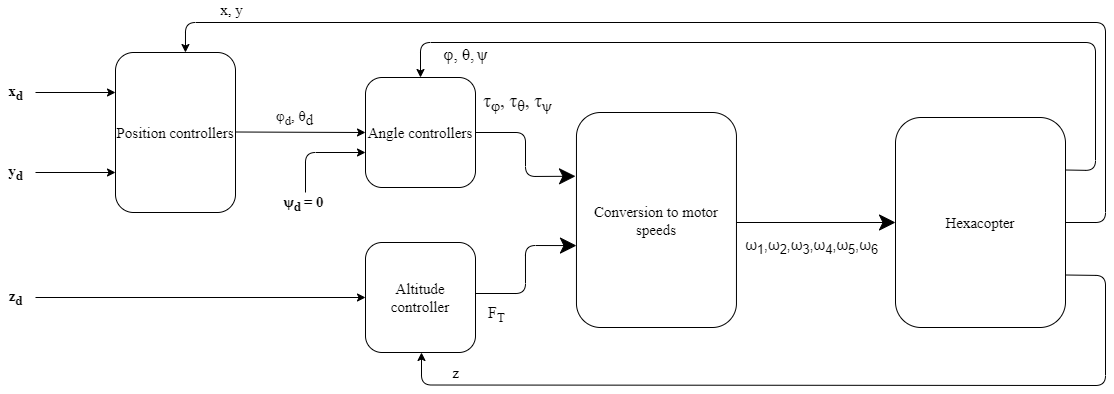
\includegraphics[width=\columnwidth]{PID_Hexacopter.PNG}%
	\caption{Complete PD control system block diagram}%
	\label{fig:PID_Hexacopter}%
\end{figure}

The gains of each controller were tuned independently using the Simulink Design Optimization Package. The Response Optimizer app within this package uses gradient descent to tune the controller gains in order to achieve the specified performance of step response. The gains achieved using this method are given in Table \ref{table:PID_Gains}.
\begin{table}[htb]
\begin{center}
\begin{tabular}{||c|c|c||} 
 \hline
 Controller & Gain & Value\\ [0.5ex] 
 \hline\hline
 \multirow{2}{7em}{Roll Angle}& K\textsubscript{P,$\phi$} & 2.688 \\ 
 \cline{2-3}
  &K\textsubscript{D,$\phi$} & 2.385 \\
 \hline
  \multirow{2}{7em}{Pitch Angle}& K\textsubscript{P,$\theta$} & 2.688 \\
 \cline{2-3}
  &K\textsubscript{D,$\theta$} & 2.385 \\
 \hline
 \multirow{2}{7em}{Yaw Angle}& K\textsubscript{P,$\psi$} & 0.759 \\
 \cline{2-3}
 &K\textsubscript{D,$\psi$} & 0.664 \\
 \hline
 \multirow{2}{7em}{x Position}& K\textsubscript{P,$x$} & 3.322 \\
 \cline{2-3}
 &K\textsubscript{D,$x$} & 2.020 \\
 \hline
 \multirow{2}{7em}{y Position}& K\textsubscript{P,$y$} & 1.471 \\
 \cline{2-3}
 &K\textsubscript{D,$y$} & 1.681 \\
 \hline
 \multirow{2}{7em}{z Position}& K\textsubscript{P,$z$} & 218.4 \\
 \cline{2-3}
 &K\textsubscript{D,$z$} & 162.5 \\
 \hline
\end{tabular}
\caption{PD controller gains}
\label{table:PID_Gains}
\end{center}
\end{table}

\FloatBarrier

\subsection{Preliminary Results}
The PD control system was implemented in Simulink and its ability to stabilise the Euler angles from significant initial conditions was tested. The system simultaneously stabilises the position and counteracts any deviations from the origin, as seen in \figref{fig:PID_Stabilise}.
\begin{figure}[htb]
\begin{center}
	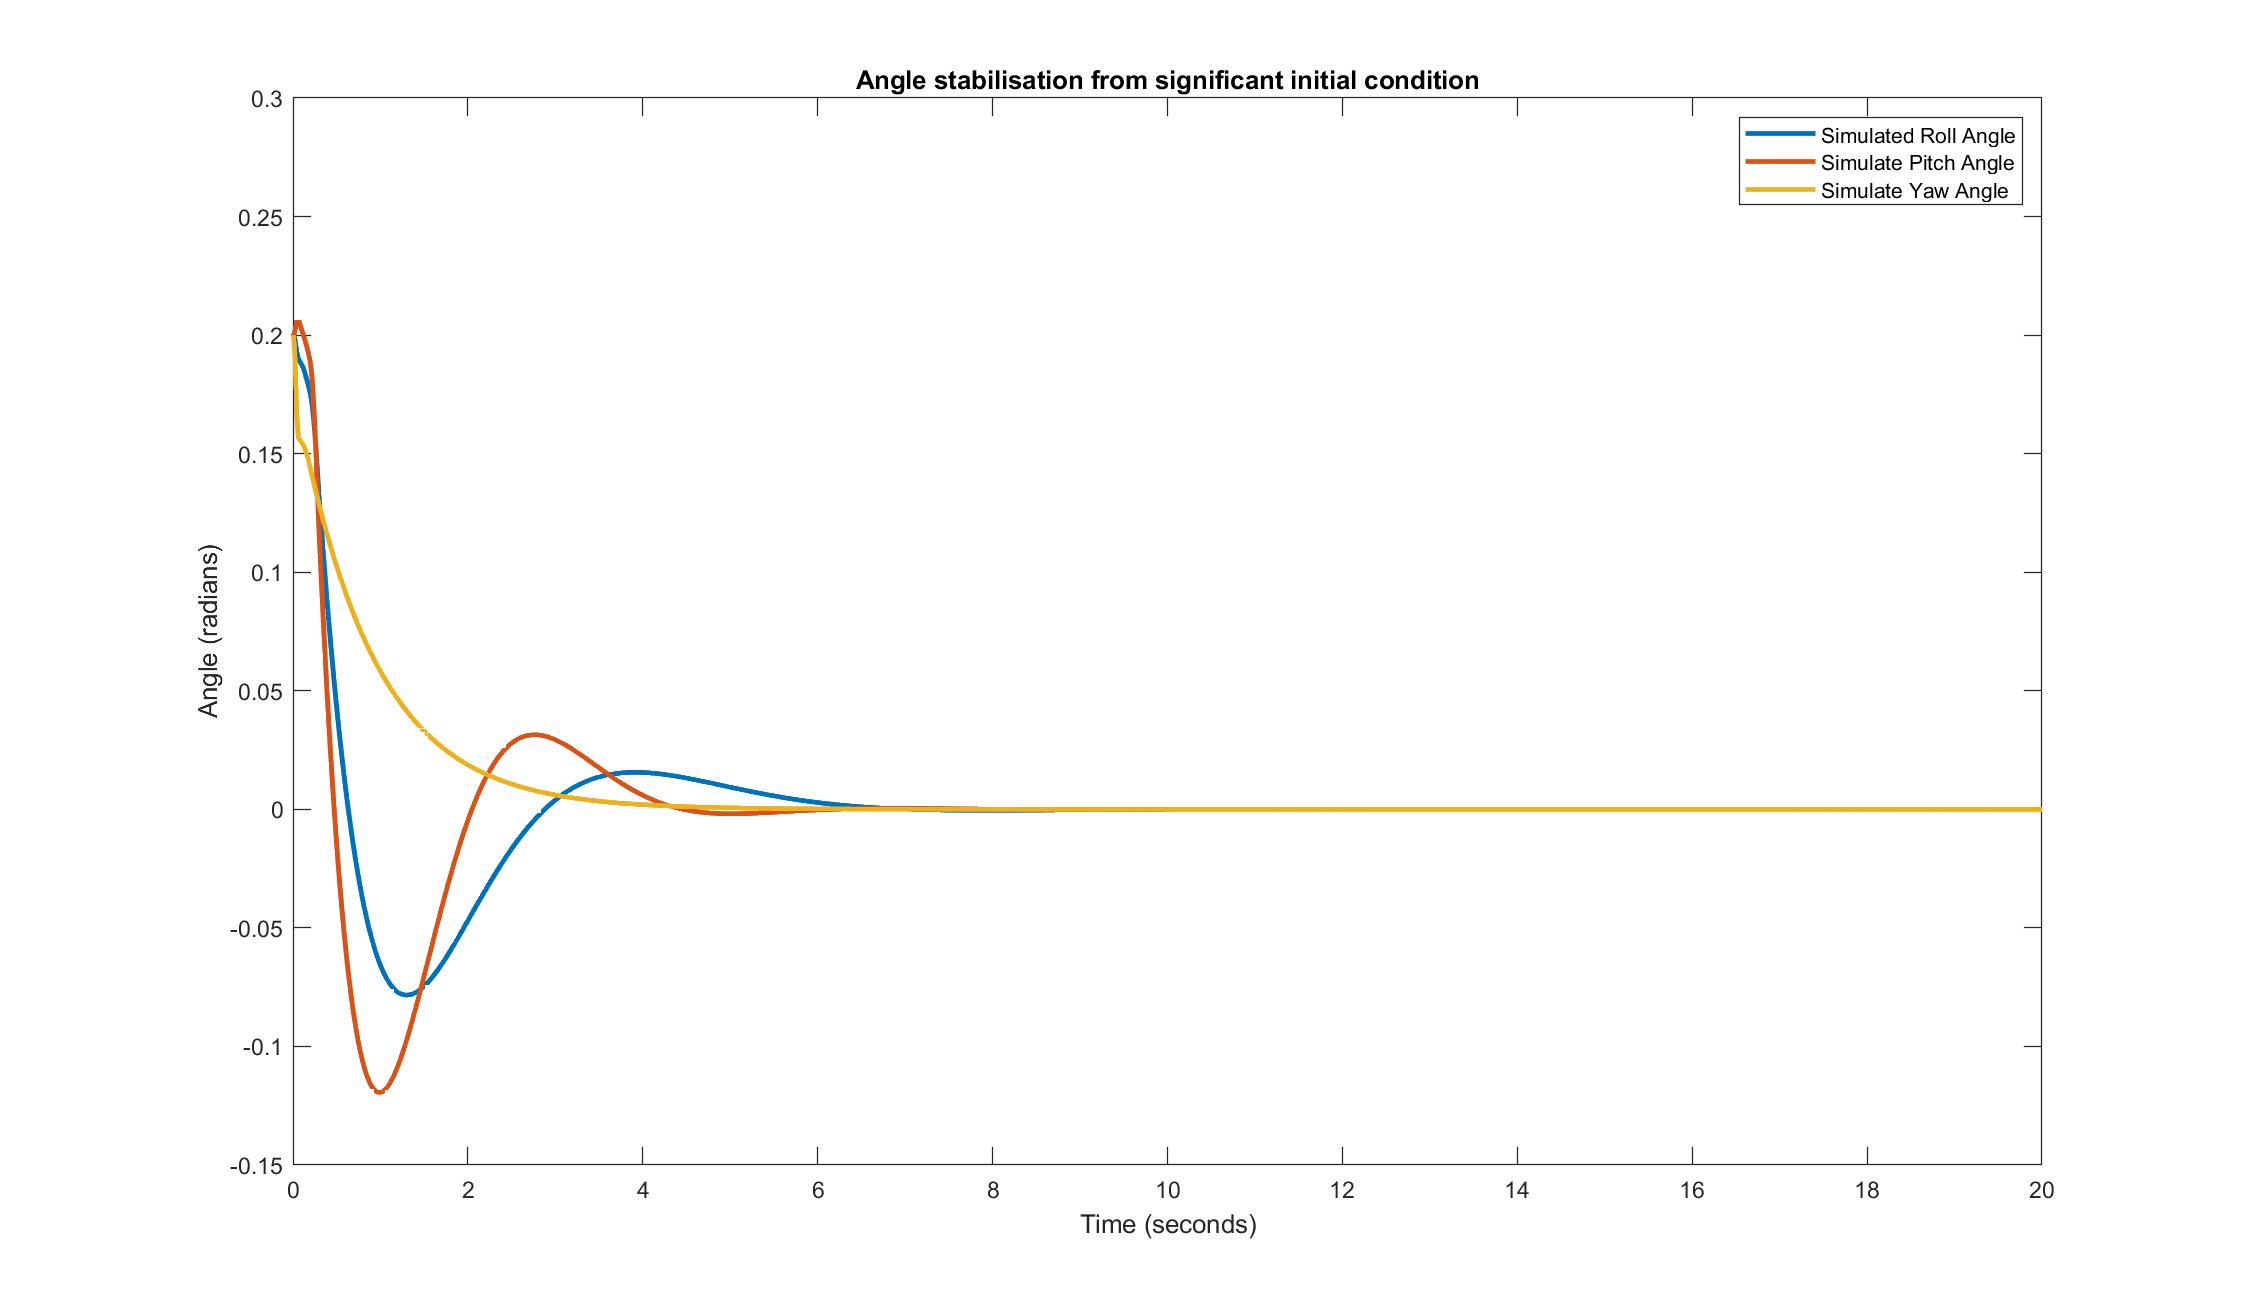
\includegraphics[width=70mm]{/PID_Results/Stabilise_Angles}
	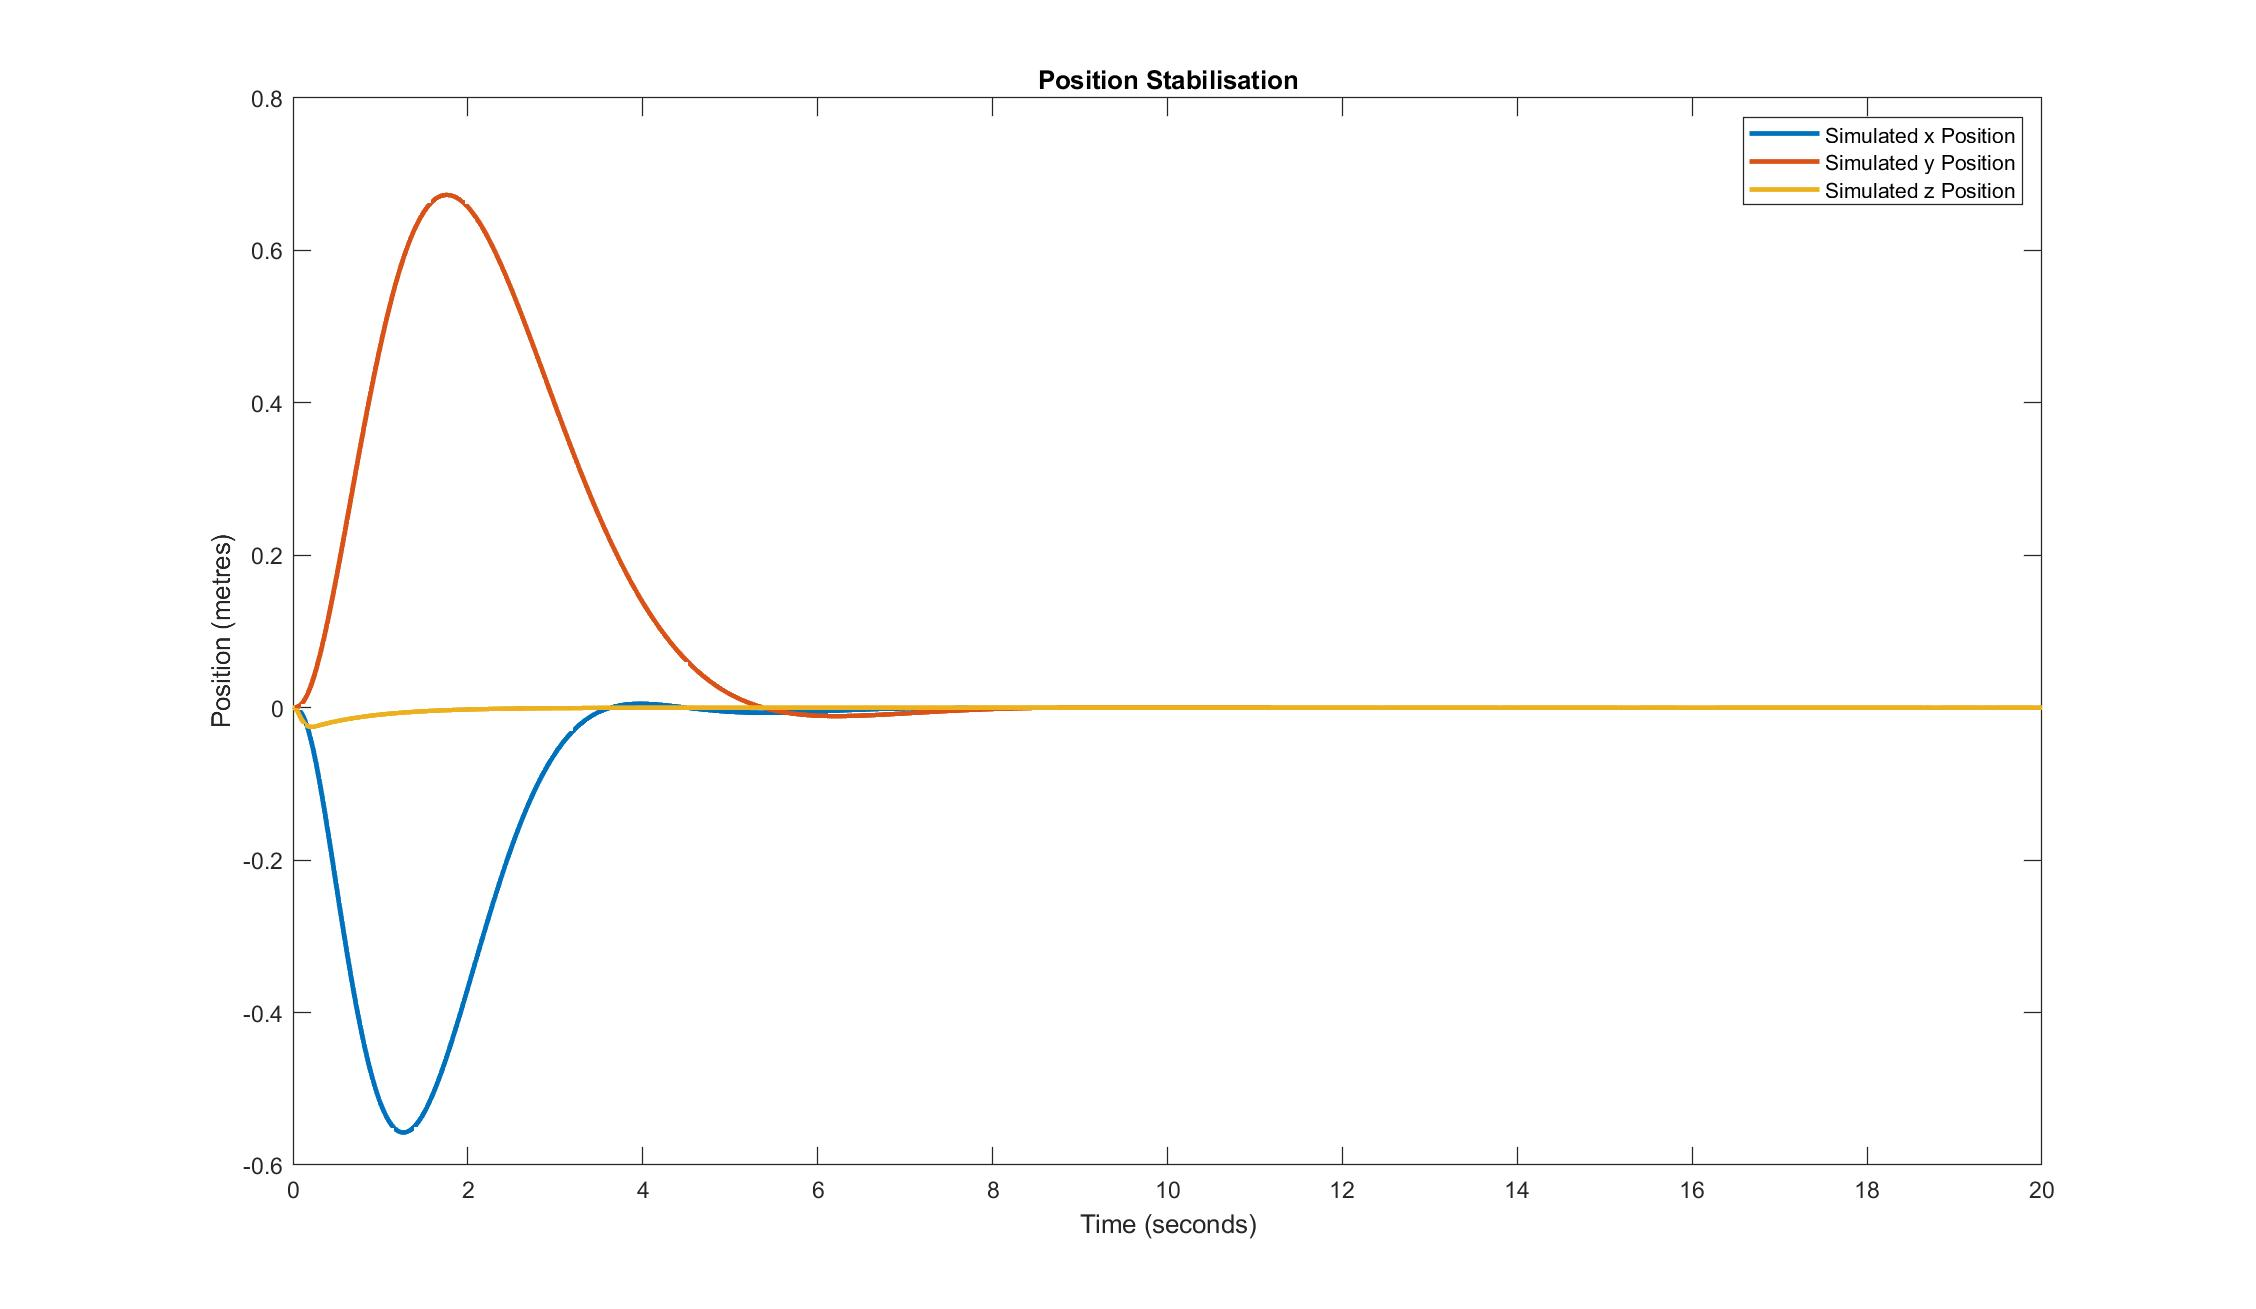
\includegraphics[width=70mm]{/PID_Results/Stabilise_Position}%
	\end{center}
	\caption{PD system stabilisation from significant initial angles}%
	\label{fig:PID_Stabilise}%
\end{figure}

The system tracking capabilities were also tested with step reference inputs. The step responses for roll angle, x position and altitude can be seen in \figref{fig:PID_Results}. The step response of the other angles ($\theta$, $\psi$) are very similar to the roll angle response and the y position response is similar to that of the x position, therefore these responses are not shown for brevity.
\begin{figure}[htb]
\begin{center}
	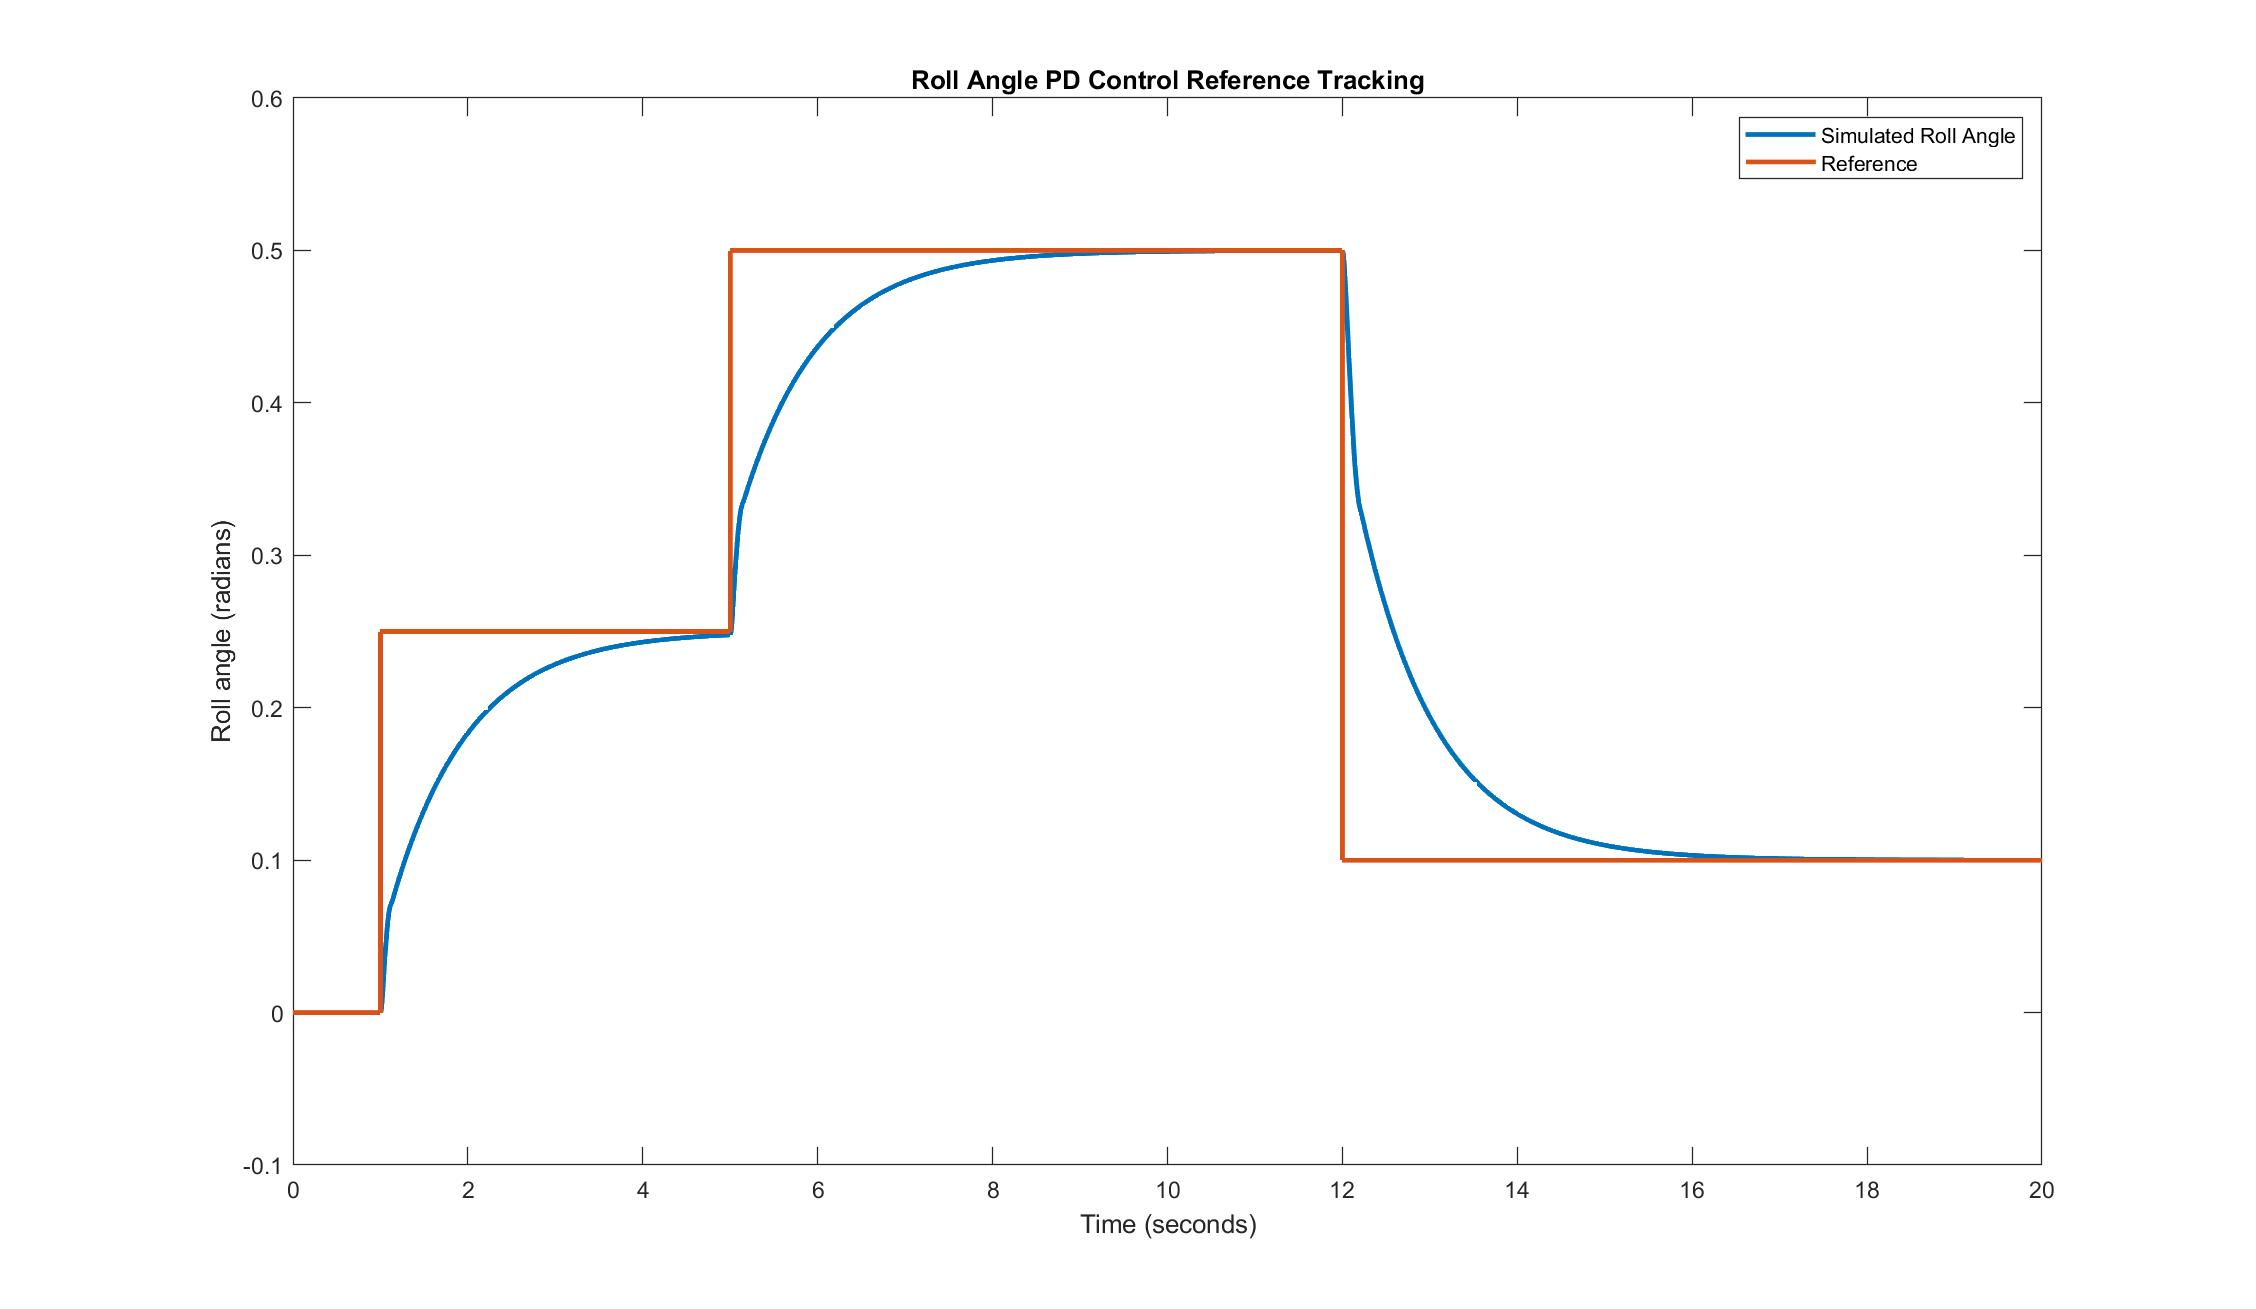
\includegraphics[width=75mm]{/PID_Results/PhiTracking_Steps2}\\
	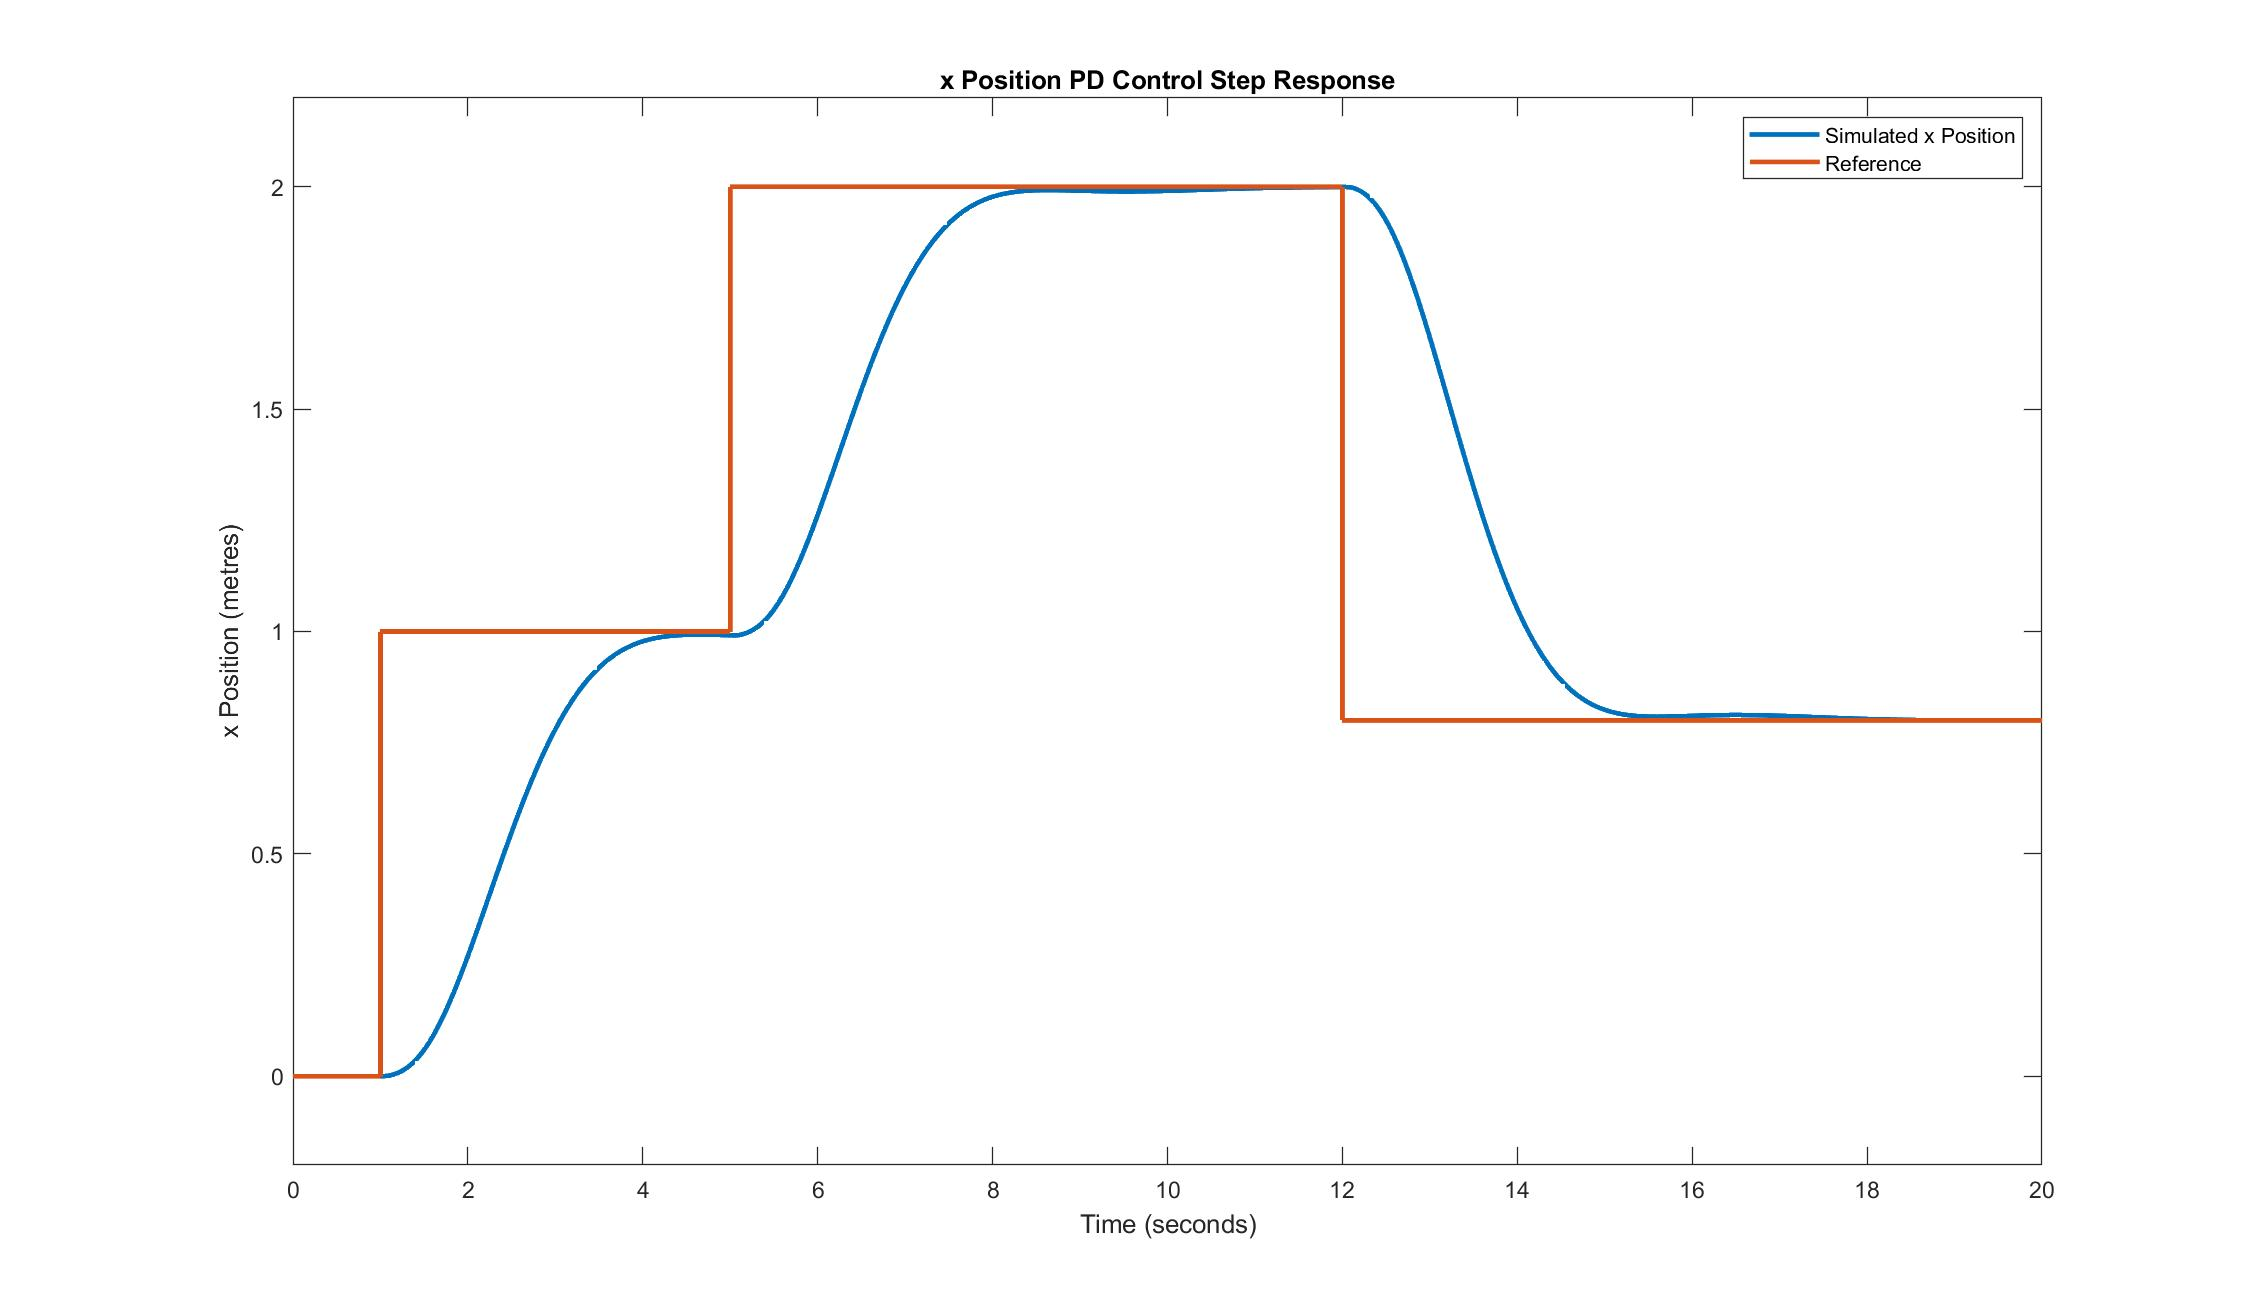
\includegraphics[width=75mm]{/PID_Results/xTracking_Steps2}%
	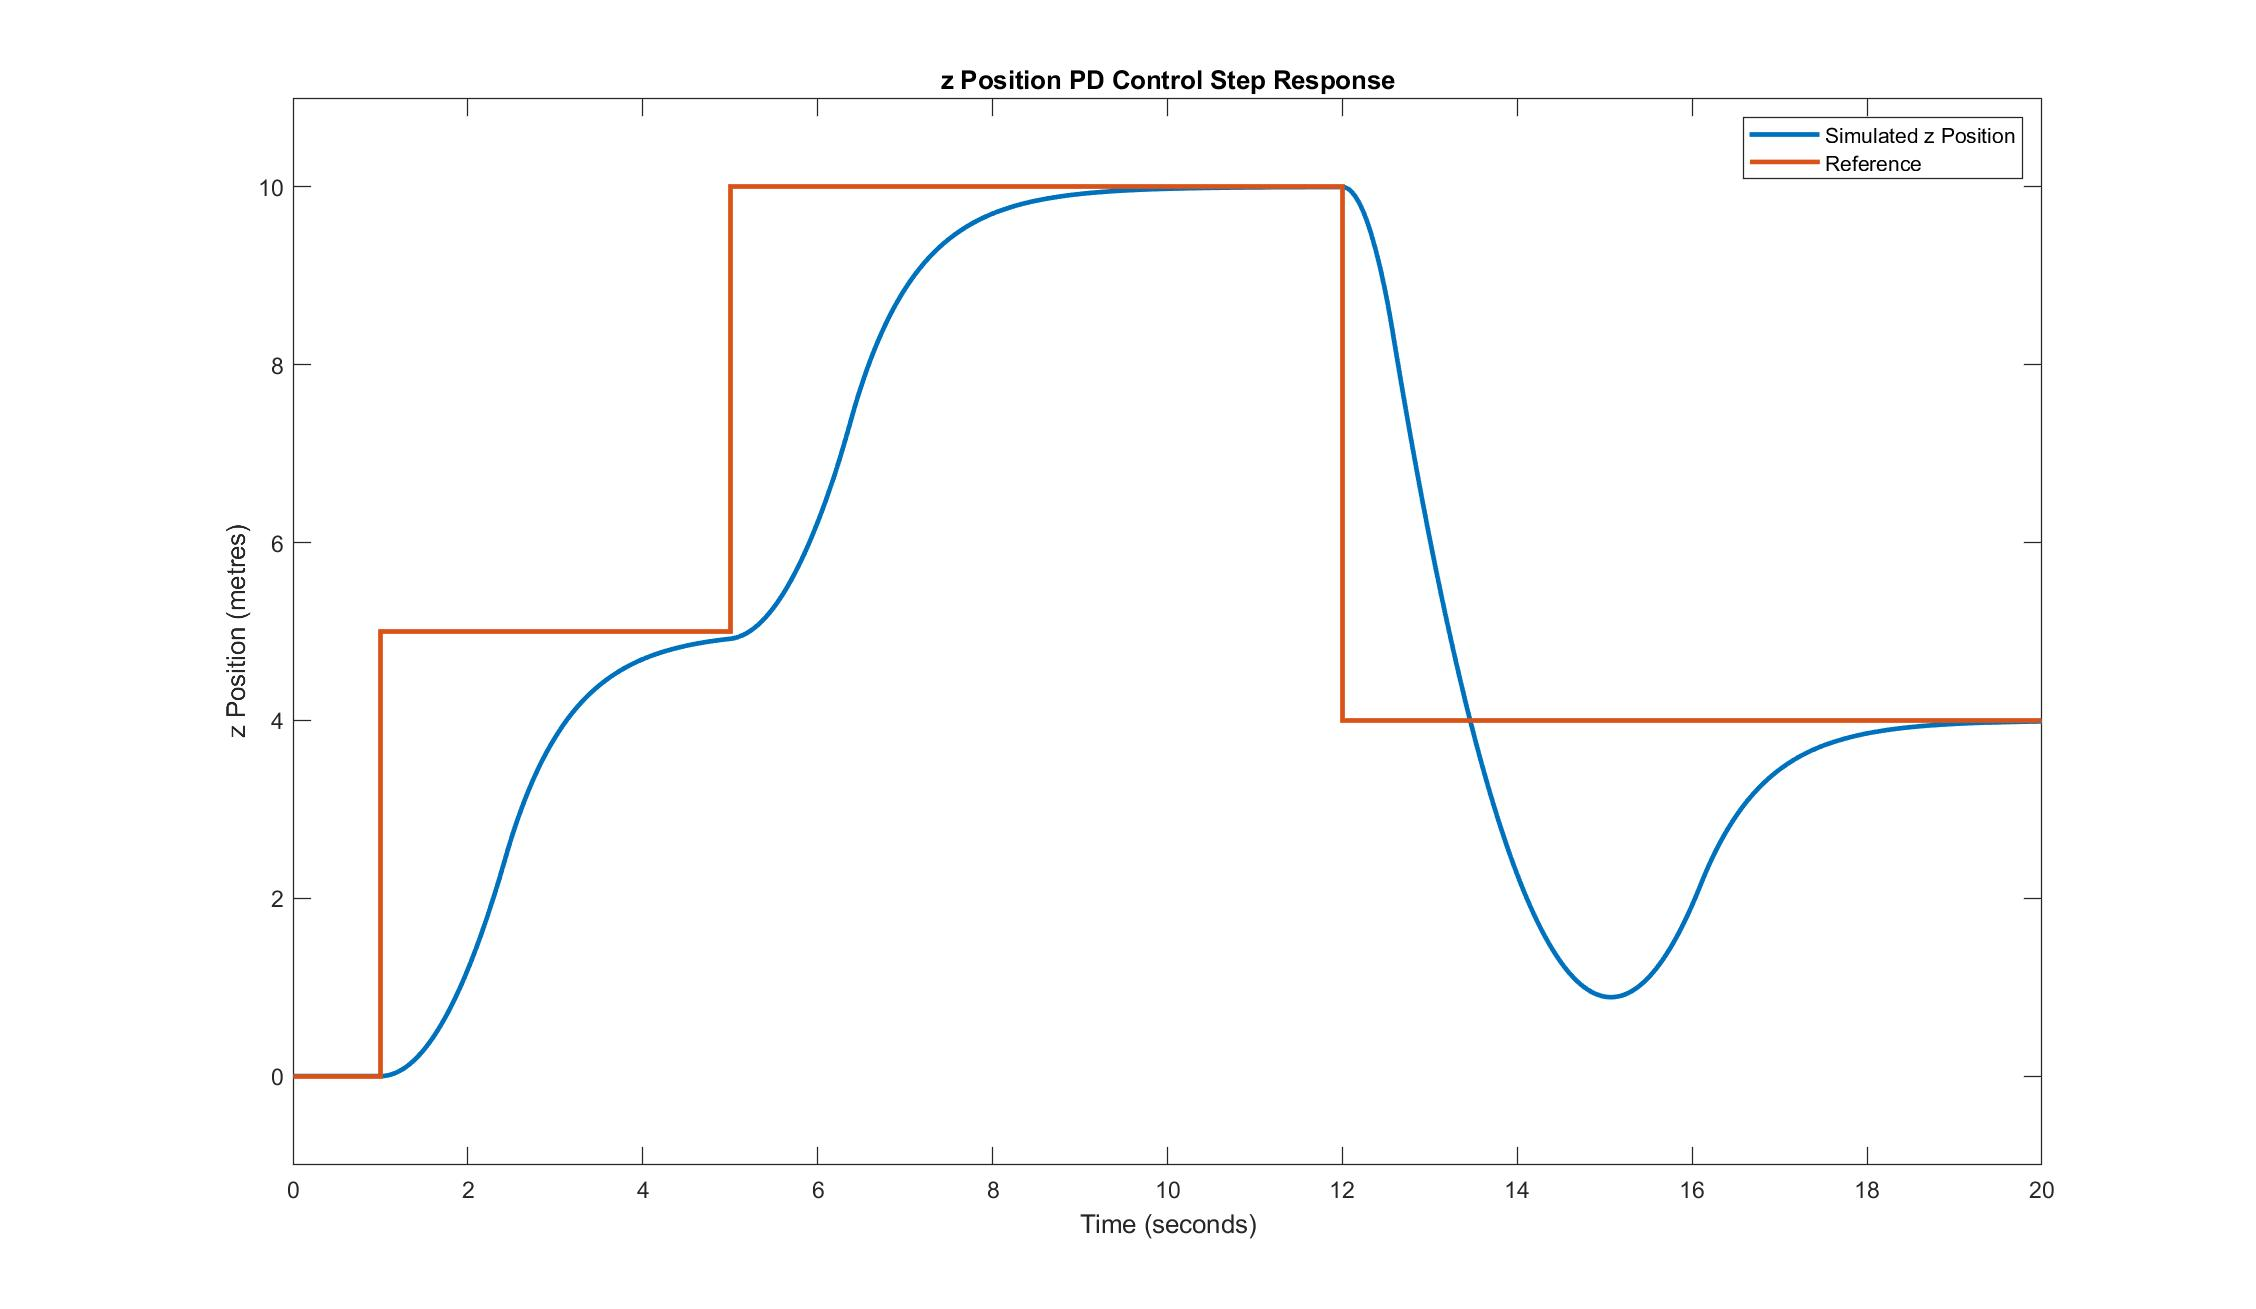
\includegraphics[width=75mm]{/PID_Results/zTracking_Steps2}%
	\end{center}
	\caption{PD system step responses}%
	\label{fig:PID_Results}%
\end{figure}
The control system was also shown to be reasonably effective in tracking a sinusoidal position command, as shown in \figref{fig:PID_Sine}.
\begin{figure}[htb]
\begin{center}
	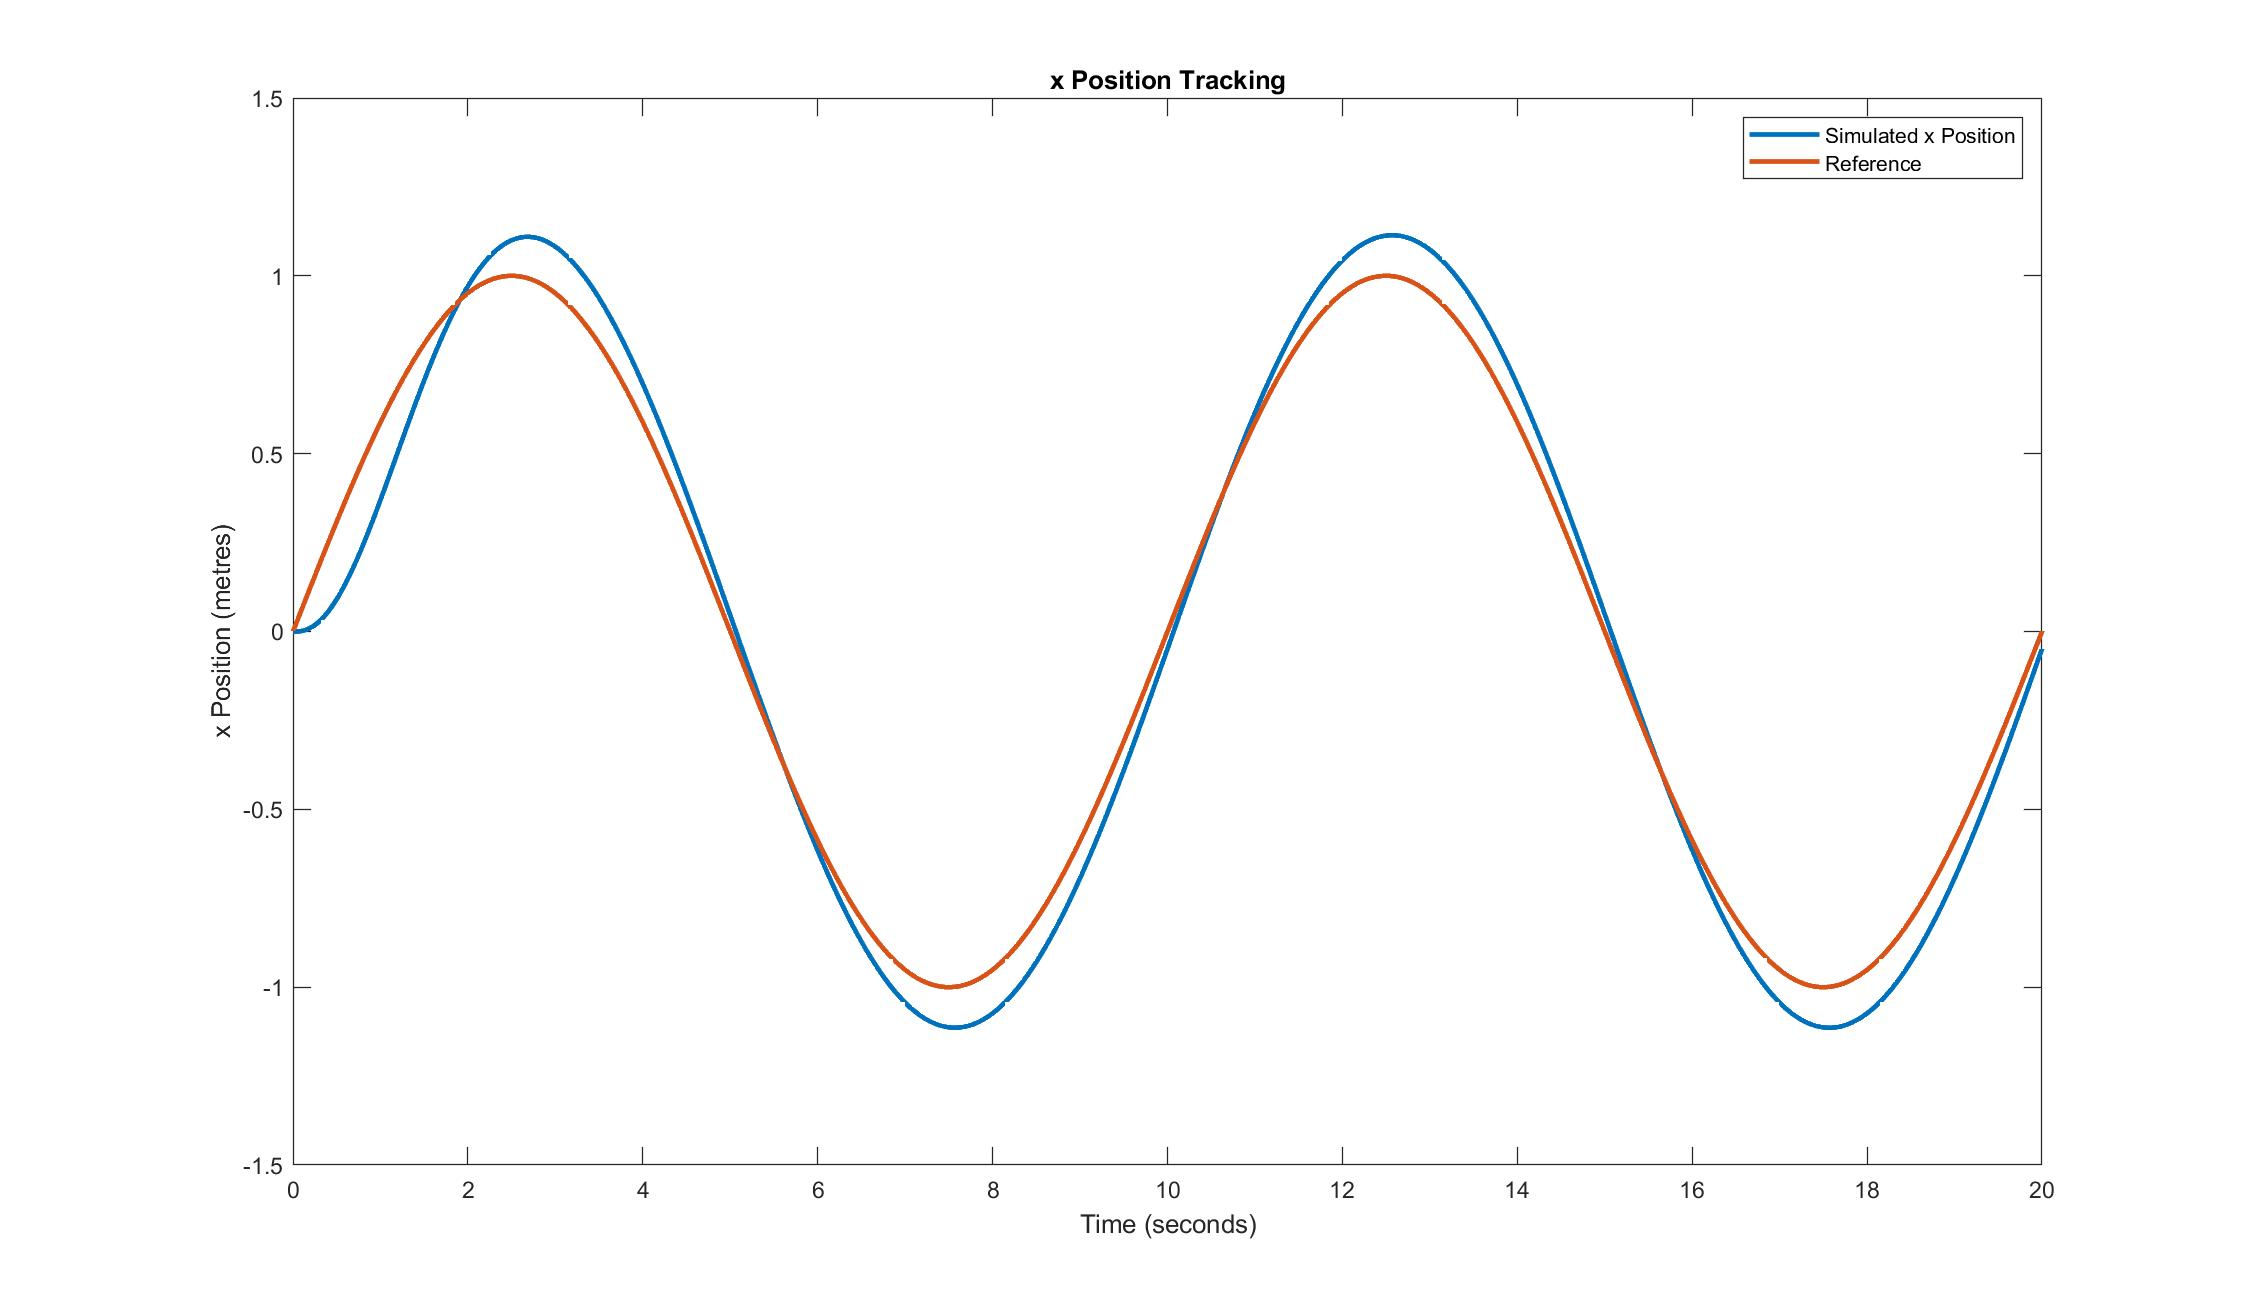
\includegraphics[width=80mm]{/PID_Results/xTracking_Sine2.jpg}%
	\end{center}
	\caption{PD Position tracking}%
	\label{fig:PID_Sine}%
\end{figure}

The results show that this system is effective in stabilising the aircraft around a hovering point in the absence of major disturbances. It is also able to respond to relatively small positional step commands. However, this control method is limited since it neglects the nonlinearities of the physical system. For example, it is ineffective with a non-zero yaw angle due to approximations made in the simplification of the model. This limits the manoeuvrability of the vehicle and makes the control system unsuitable for many applications. For example, many UAV platforms are able to be equipped with a camera fixed to the underside of the vehicle body and the yaw angle is used to direct the camera field of view to points of interest.  The system is also prone to saturation when subject to large step commands.

\FloatBarrier
\section{Backstepping Control}
In order to improve upon the performance of the previous controller, the recursive Lyapunov-based control method known as backstepping will be applied to the multi-rotor system. The mathematical background of this method is discussed in Section \ref{section:BacksteppingBackground}.
\subsection{Simplified State Space Model}
The states used by the backstepping controller will be each of the positions in the Earth frame as well as their respective velocities. In order to simplify notation, the states will be referred to as $x_{i}$ and are defined as:
\begin{equation}\label{eqn:stateDef}
\textbf{\textit{x}}=
\begin{bmatrix}
x_{1}\\
x_{2}\\
x_{3}\\
x_{4}\\
x_{5}\\
x_{6}\\
x_{7}\\
x_{8}\\
x_{9}\\
x_{10}\\
x_{11}\\
x_{12}
\end{bmatrix}
=
\begin{bmatrix}
\phi\\
\dot{\phi}\\
\theta\\
\dot{\theta}\\
\psi\\
\dot{\psi}\\
x\\
\dot{x}\\
y\\
\dot{y}\\
z\\
\dot{z}
\end{bmatrix}
\end{equation}

As seen in Section \ref{section:SimpleModel}, the state space model which was presented in Section \ref{section:ModelDynamics}, is able to be greatly simplified by making a number of assumptions. For the purposes of this controller, the small angle approximation will be used in order to simplify the relationship between the torques and the Euler angles. That is, the relationship in \eqref{eqn:simpleState1} will be assumed true. Applying this to \eqref{eqn:state3} gives the following:

\begin{equation}
\begin{bmatrix}
\dot{x}_{2}\\
\dot{x}_{4}\\
\dot{x}_{6}
\end{bmatrix}
=
\begin{bmatrix}
a_{1}x_{4}x_{6}+b_{1}\tau_{\phi}\\
a_{2}x_{2}x_{6}+b_{2}\tau_{\theta}\\
a_{3}x_{2}x_{4}+b_{3}\tau_{\psi}
\end{bmatrix}
\end{equation}
with $a_{1}=\frac{I_{yy}-I_{zz}}{I_{xx}}$, $a_{2}=\frac{I_{zz}-I_{xx}}{I_{yy}}$, $a_{3}=\frac{I_{xx}-I_{yy}}{I_{zz}}$, $b_{1}=\frac{1}{I_{xx}}$, $b_{2}=\frac{1}{I_{yy}}$, $b_{3}=\frac{1}{I_{zz}}$. Also, the second order translational dynamics established in \eqref{eqn:additionalState2} are used for this controller. Now, the simplified state space model may be expressed:

\begin{equation}\label{eqn:simpleStateModel}
\begin{bmatrix}
\dot{x}_{1}\\
\dot{x}_{2}\\
\dot{x}_{3}\\
\dot{x}_{4}\\
\dot{x}_{5}\\
\dot{x}_{6}\\
\dot{x}_{7}\\
\dot{x}_{8}\\
\dot{x}_{9}\\
\dot{x}_{10}\\
\dot{x}_{11}\\
\dot{x}_{12}
\end{bmatrix}
=
\begin{bmatrix}
x_{2}\\
a_{1}x_{4}x_{6}+b_{1}\tau_{\phi}\\
x_{4}\\
a_{2}x_{2}x_{4}+b_{2}\tau_{\theta}\\
x_{6}\\
a_{3}x_{2}x_{4}+b_{3}\tau_{\psi}\\
x_{8}\\
[-cos(x_{1})sin(x_{3})cos(x_{5})-sin(x_{1})sin(x_{5})]\frac{F_{T}}{m}\\
x_{10}\\
[-cos(x_{1})sin(x_{3})sin(x_{5})+sin(x_{1})cos(x_{5})]\frac{F_{T}}{m}\\
x_{12}\\
[cos(x_{1})cos(x_{3})]\frac{F_{T}}{m}-g
\end{bmatrix}
\end{equation}

\subsection{Attitude Control}
Consider the tracking error of the roll angle, i.e. the first state:
\[z_{1}= x_{1d}-x_{1}\]

Choose a candidate Lyapunov function such that it is positive definite:
\[V(z_{1})=\frac{1}{2}z_{1}^{2}\]
Taking its derivative gives:

\[\dot{V}(z_{1})=z_{1}\dot{z}_{1}\]

A control Lyapunov function must have a negative definite derivative, therefore \(\dot{z_{1}}\) is chosen to be \(-K_{1}z_{1}\) with constant gain \(K_{1}>0\). This gives the following result:
\[\dot{V}(z_{1})=-K_{1}z_{1}^{2}\]
Now, take the derivative of \(z_{1}\) and substitute our chosen value.
\begin{equation*}
\begin{split}
\dot{z}_{1}&=\dot{x}_{1d}-\dot{x}_{1}\\
-K_{1}z_{1}&=\dot{x}_{1d}-x_{2}\\
\end{split}
\end{equation*}
Now, choose a virtual control \(x_{2d}\) to satisfy this relationship:
\[x_{2d}=\dot{x}_{1d}+K_{1}z_{1}\]
Now consider the tracking error of the second state:
\begin{equation*}
\begin{split}
z_{2}&=x_{2d}-x_{2}\\
&=\dot{x}_{1d}+K_{1}z_{1}-x_{2}
\end{split}
\end{equation*}
Now choose a second candidate Lyapunov function:
\[V(z_{1},z_{2})=\frac{1}{2}(z_{1}^2+z_{2}^2)\]
Then take its derivative:
\begin{equation*}
\begin{split}
\dot{V}(z_{1},z_{2})&=\dot{V}(z_{1})+z_{2}\dot{z}_{2}\\
&=-K_{1}z_{1}^{2}+z_{2}\dot{z}_{2}
\end{split}
\end{equation*}
Now to ensure \(\dot{V}(z_{1},z_{2})\) is negative definite, choose \(\dot{z}_{2}=-K_{2}z_{2}\) with constant \(K_{2}>0\). This gives the following result:
\begin{equation*}
\begin{split}
\dot{z}_{2}&=\ddot{x}_{1d}+K_{1}\dot{z}_{1}-\dot{x}_{2}\\
-K_{2}z_{2}&=\ddot{x}_{1d}+K_{1}(\dot{x}_{1d}-x_{2})-a_{1}x_{4}x_{6}-b_{1}\tau_{\phi}
\end{split}
\end{equation*}
Using this result, it is possible to choose a control value for the input \(\tau_{\phi}\) which will stabilise the roll angle:
\begin{equation}\label{eqn:BackstepPhiLaw}
\tau_{\phi}=\frac{1}{b_{1}}(\ddot{x}_{1d}+K_{1}(\dot{x}_{1d}-x_{2})-a_{1}x_{4}x_{6}+K_{2}z_{2})
\end{equation}
The same steps can be followed to stabilise both the pitch and yaw angles with control inputs \(\tau_{\theta}\) and \(\tau_{\psi}\) respectively. These control laws are given in \eqref{eqn:BackstepAngleLaws}.

\begin{equation}\label{eqn:BackstepAngleLaws}
\begin{split}
\tau_{\theta}&=\frac{1}{b_{2}}\left(\ddot{x}_{3d}+K_{3}(\dot{x}_{3d}-x_{4})-a_{2}x_{2}x_{6}+K_{4}z_{4}\right)\\
\tau_{\psi}&=\frac{1}{b_{3}}\left(\ddot{x}_{5d}+K_{5}(\dot{x}_{5d}-x_{6})-a_{3}x_{2}x_{4}+K_{6}z_{6}\right)
\end{split}
\end{equation}


\subsection{Position Control}
The control laws developed in the previous section successfully allow stabilisation and tracking of the vehicle's attitude, however, the objective of this control system is to allow the vehicle to track a trajectory in 3D space. First consider the tracking error of the position in the Earth frame x direction:
\[z_{7}=x_{7d}-x{7}\]
Following the same logic presented in the development of the attitude controllers, the candidate Lyapunov function is chosen as $V(z_{7})=\frac{1}{2}z_{7}^{2}$. Thus, a virtual control for $x_{8}$ is chosen to satisfy $\dot{z}_{7}=-K_{7}z_{7}$:
\[x_{8d}=\dot{x}_{7d}+K_{7}z_{7}\]

Now, consider the tracking error of the translational velocity, $z_{8}$, and its derivative:

\[
\begin{split}
z_{8}&=x_{8d}-x_{8}\\
z_{8}&=\dot{x}_{7d}+K_{7}z_{7}-x_{8}\\
\dot{z}_{8}&=\ddot{x}_{7d}+K_{7}\dot{z}_{7}-\dot{x}_{8}\\
&=\ddot{x}_{7d}+K_{7}\dot{z}_{7}-[-cos(x_{1})sin(x_{3})cos(x_{5})-sin(x_{1})sin(x_{5})]\frac{F_{T}}{m}
\end{split}
\]

In order to ensure $\dot{z}_{8}=-K_{8}z_{8}$, a virtual control must be chosen. If it is assumed that the vehicle is in hovering flight and the Euler angles are stabilised around 0\textdegree, then the most logical choice of variable for a virtual control is the pitch angle ($x_{3}$). Thus, the virtual control $x_{3d}$ in \eqref{eqn:XPosContLaw} will be supplied as a desired value for the attitude controller developed in the previous section. 
\begin{equation}\label{eqn:XPosContLaw}
x_{3d}=sin^{-1}\left(-\frac{\frac{m}{F_{T}}[K_{8}z_{8}+\ddot{x}_{7d}+K_{7}\dot{z}_{7}]+sin(x_{1})sin(x_{5})}{cos(x_{1})cos(x_{5})}\right)
\end{equation}

The y position control law, shown in \eqref{eqn:YPosContLaw}, is developed in the same way, with the roll angle ($x_{1}$) acting as the virtual control. 
\begin{equation}\label{eqn:YPosContLaw}
x_{1d}=sin^{-1}\left(\frac{\frac{m}{F_{T}}[K_{10}z_{10}+\ddot{x}_{9d}+K_{9}\dot{z}_{9}]+cos(x_{1})sin(x_{3})sin(x_{5})}{cos(x_{5})}\right)
\end{equation}
 
The z position control law in \eqref{eqn:ZPosContLaw} is developed following the same method, with $F_{T}$ as the control input.
\begin{equation}\label{eqn:ZPosContLaw}
F_{T}=\frac{m(\ddot{x}_{11d}+K_{11}\dot{z}_{11}+K_{12}z_{12}+g)}{cos(x_{1})cos(x_{3})}
\end{equation}

\subsection{Preliminary Results}
 
The gains $K_{i}$ were tuned using the Simulink Design Optimization Package. This controller was able to stabilise the angles and positions from significant initial conditions. It was also able to travel between waypoints in 3D space. \figref{fig:Backstep_path} shows the hexacopter's path: taking off, travelling between waypoints and landing at a given location. However, this controller's response to large step inputs is unpredictable due to saturation effects. Also, note the slight steady state error in the z controller shown in \figref{fig:Backstep_posTrack}.

\begin{figure}[htb]
\begin{center}
	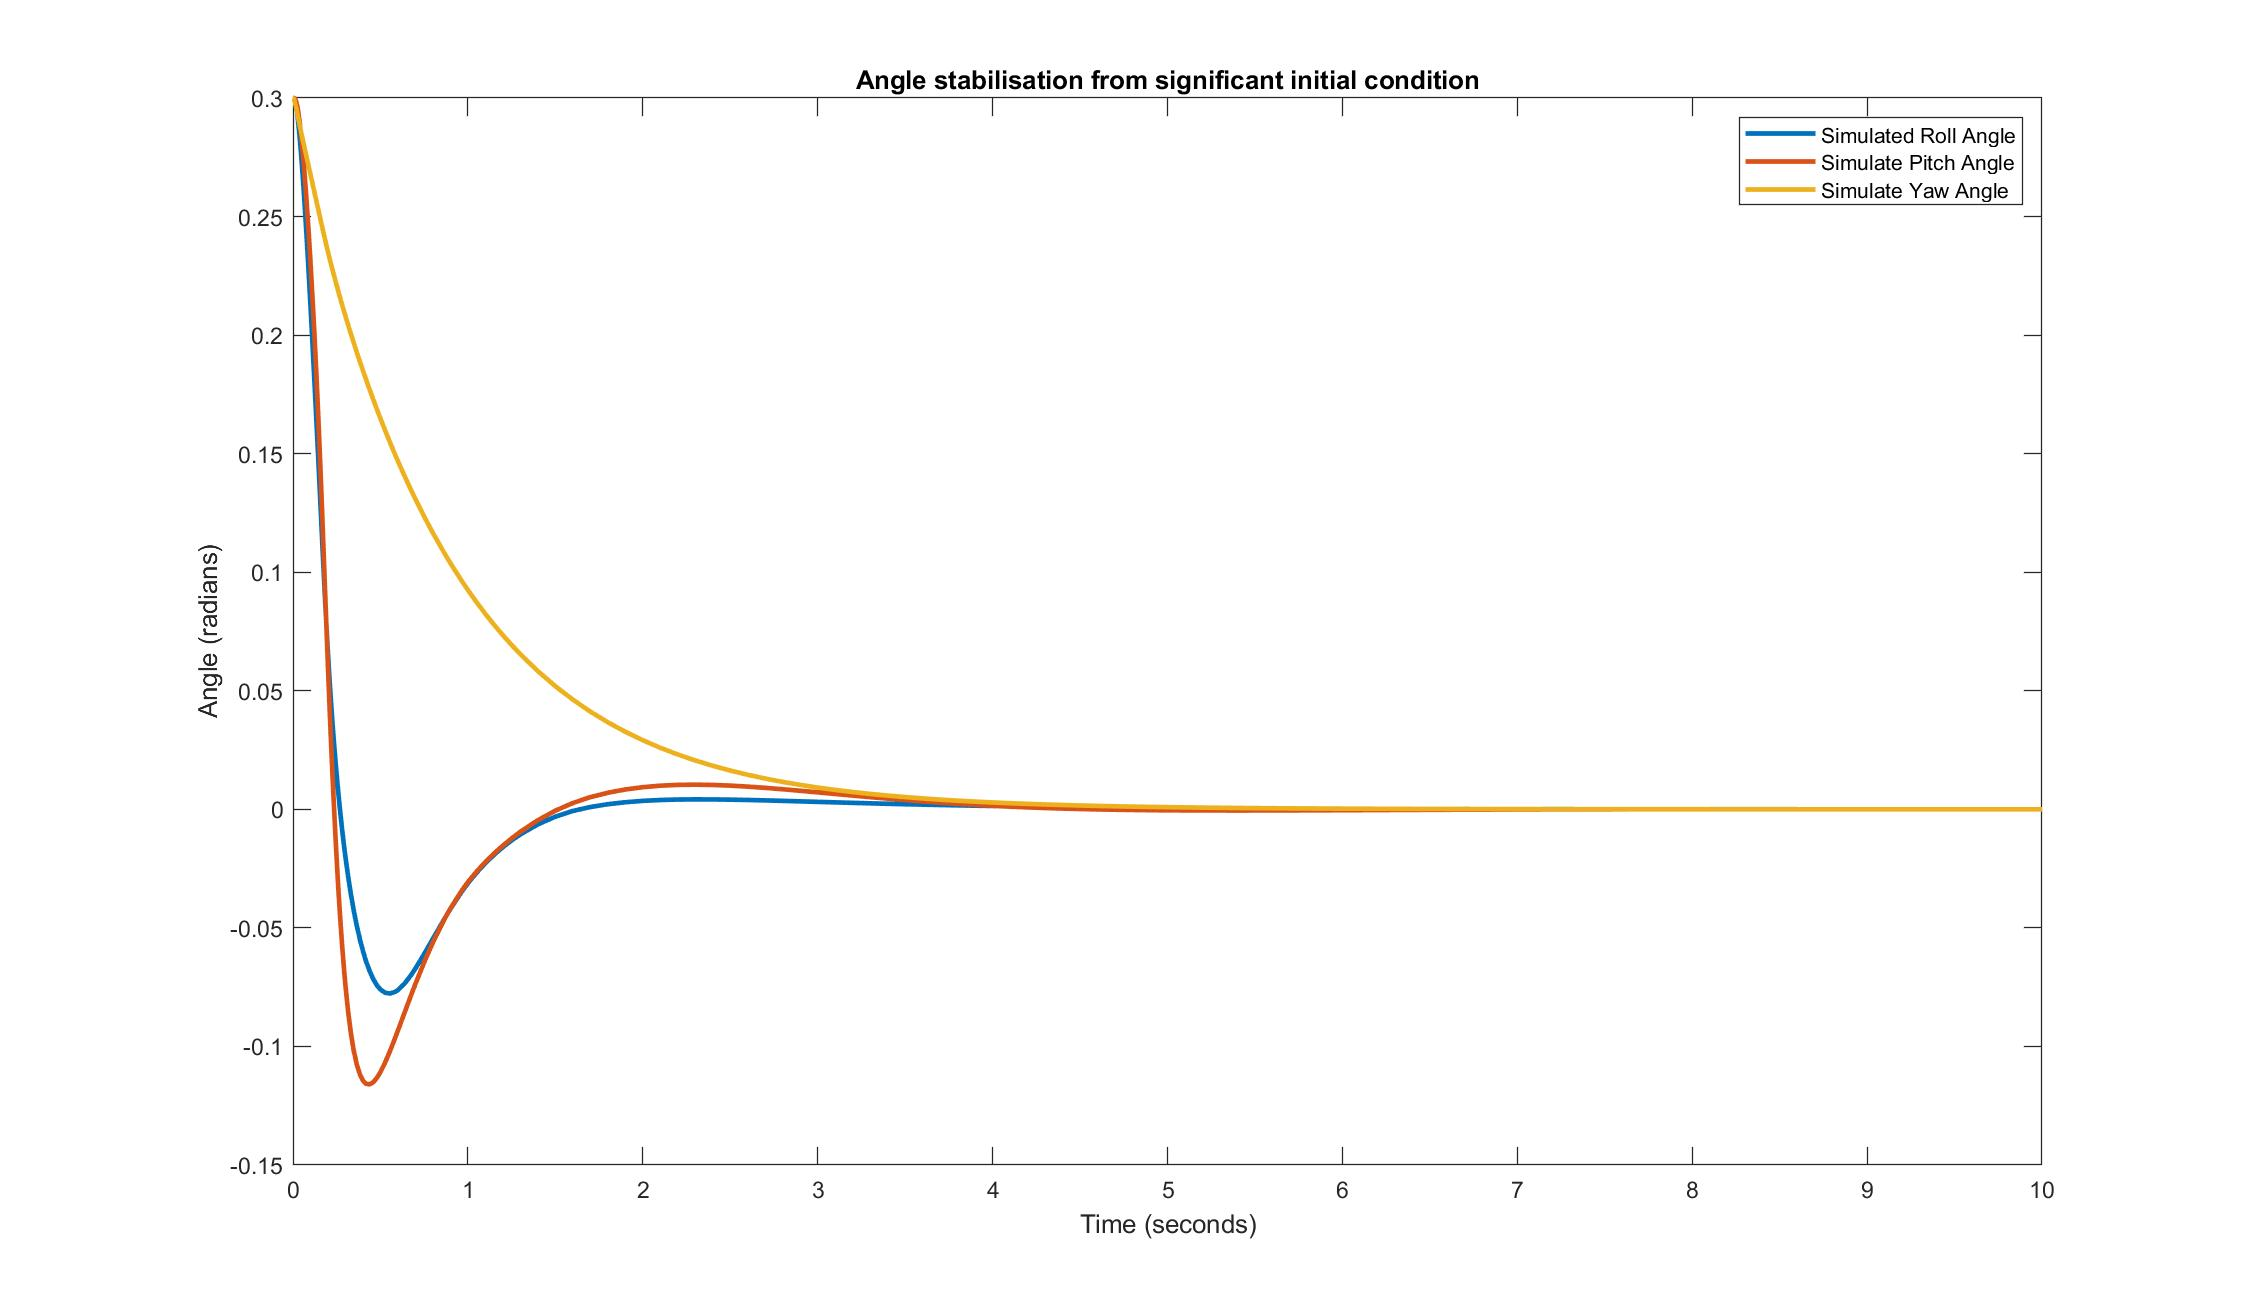
\includegraphics[width=70mm]{/Backstepping_Results/AngleStabilise}
	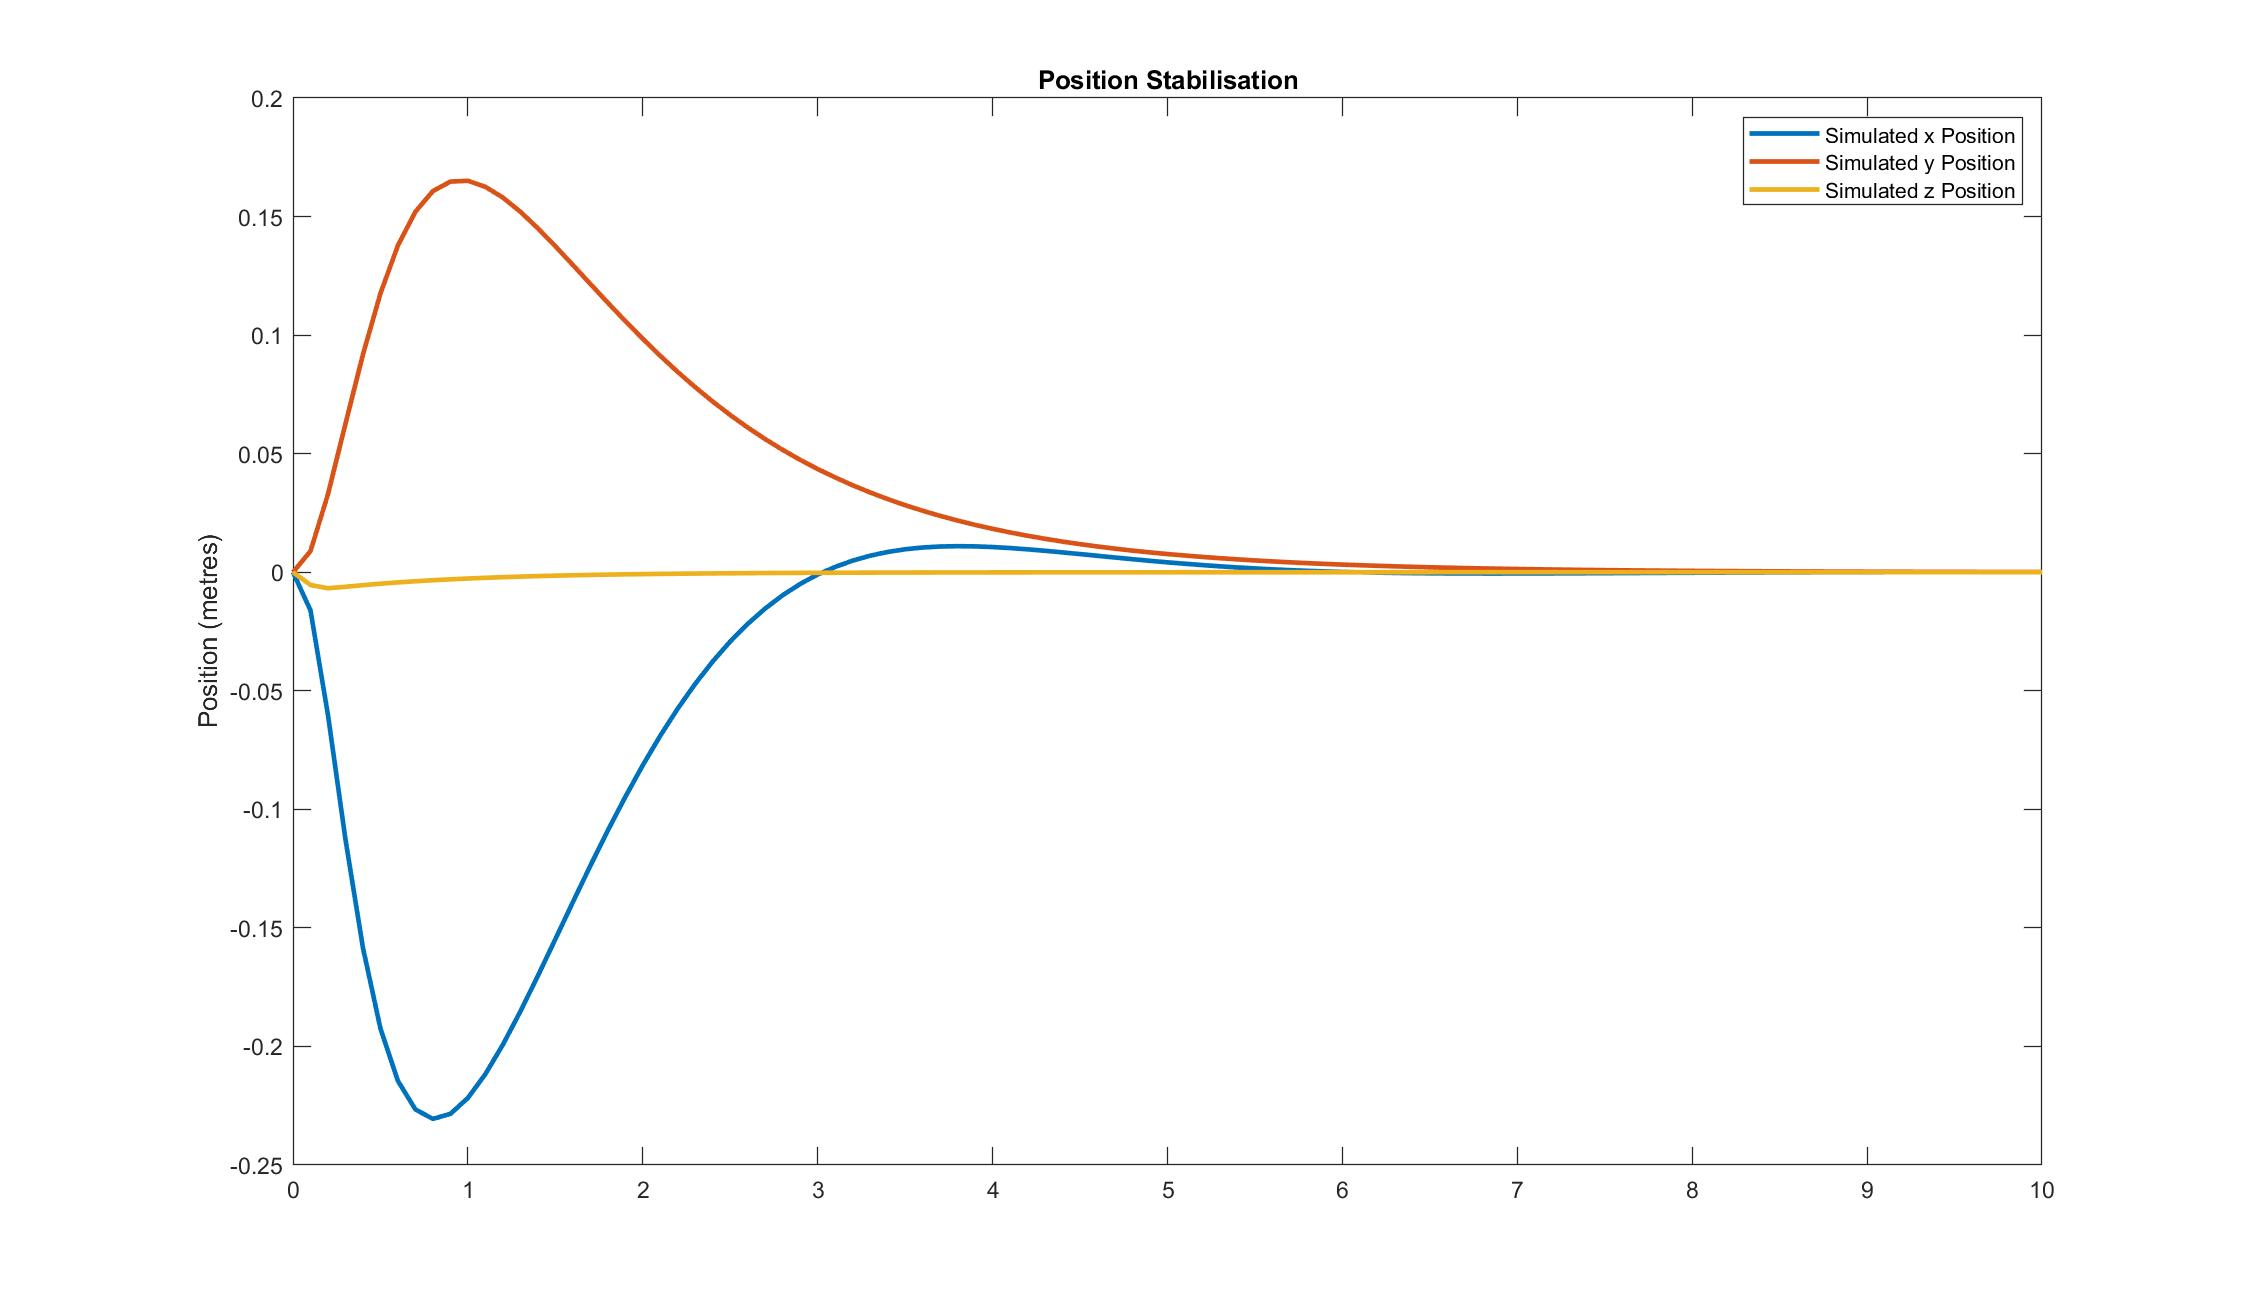
\includegraphics[width=70mm]{/Backstepping_Results/PositionStabilise}%
	\end{center}
	\caption{Backstepping system stabilisation from significant initial angles}%
	\label{fig:Backstepping_Stabilise}%
\end{figure}

\begin{figure}[htb]
\begin{center}
	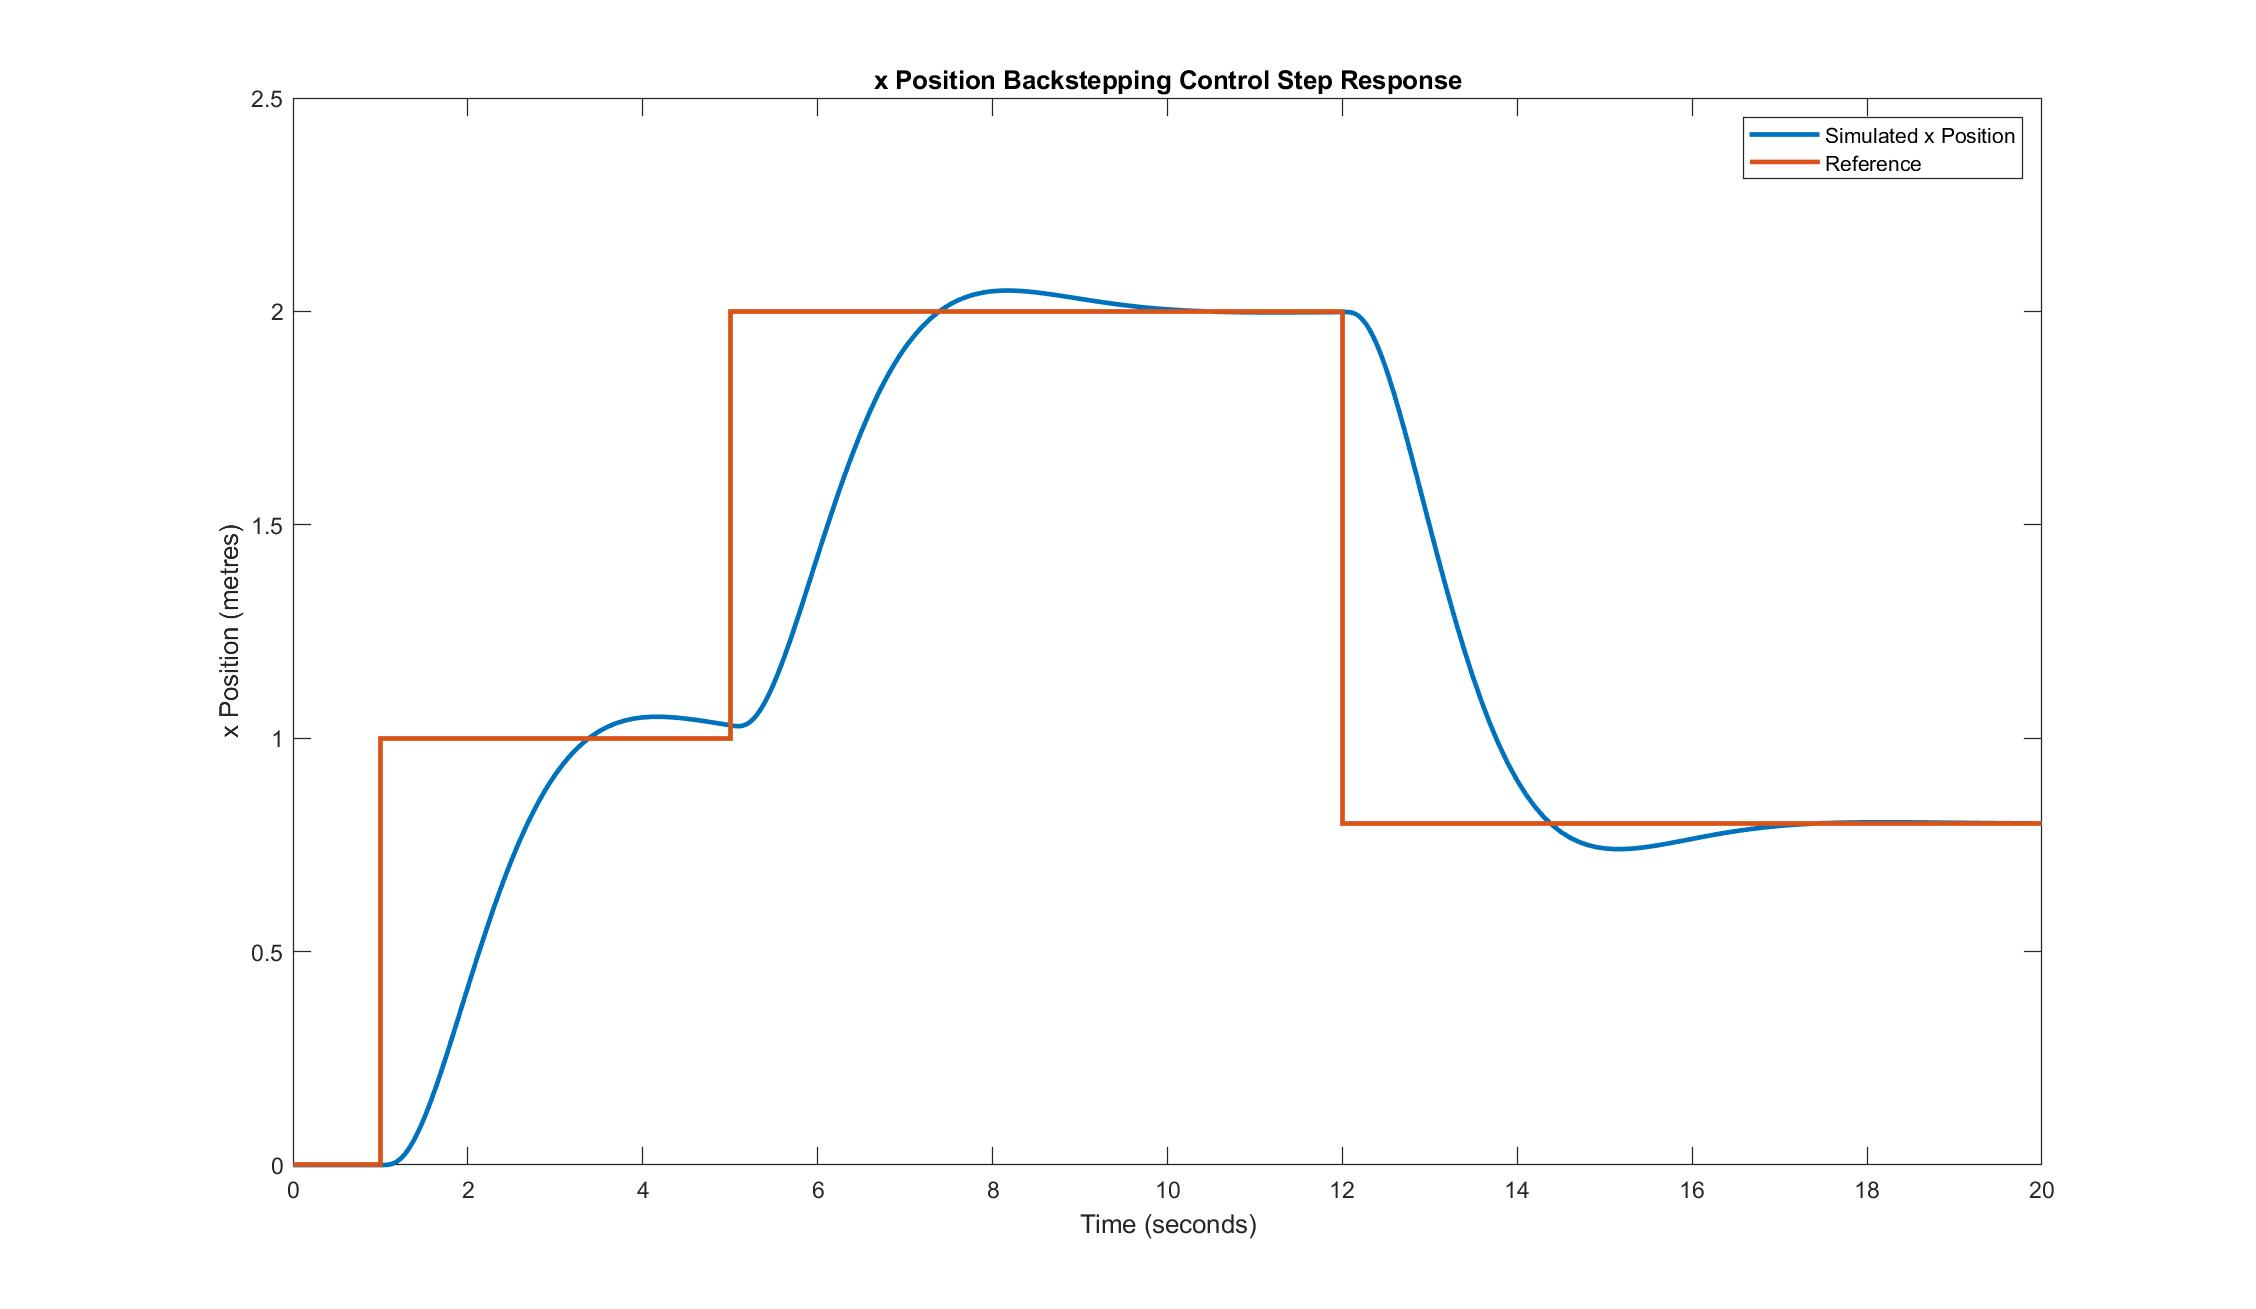
\includegraphics[width=70mm]{/Backstepping_Results/xTracking_Steps1.jpg}%
	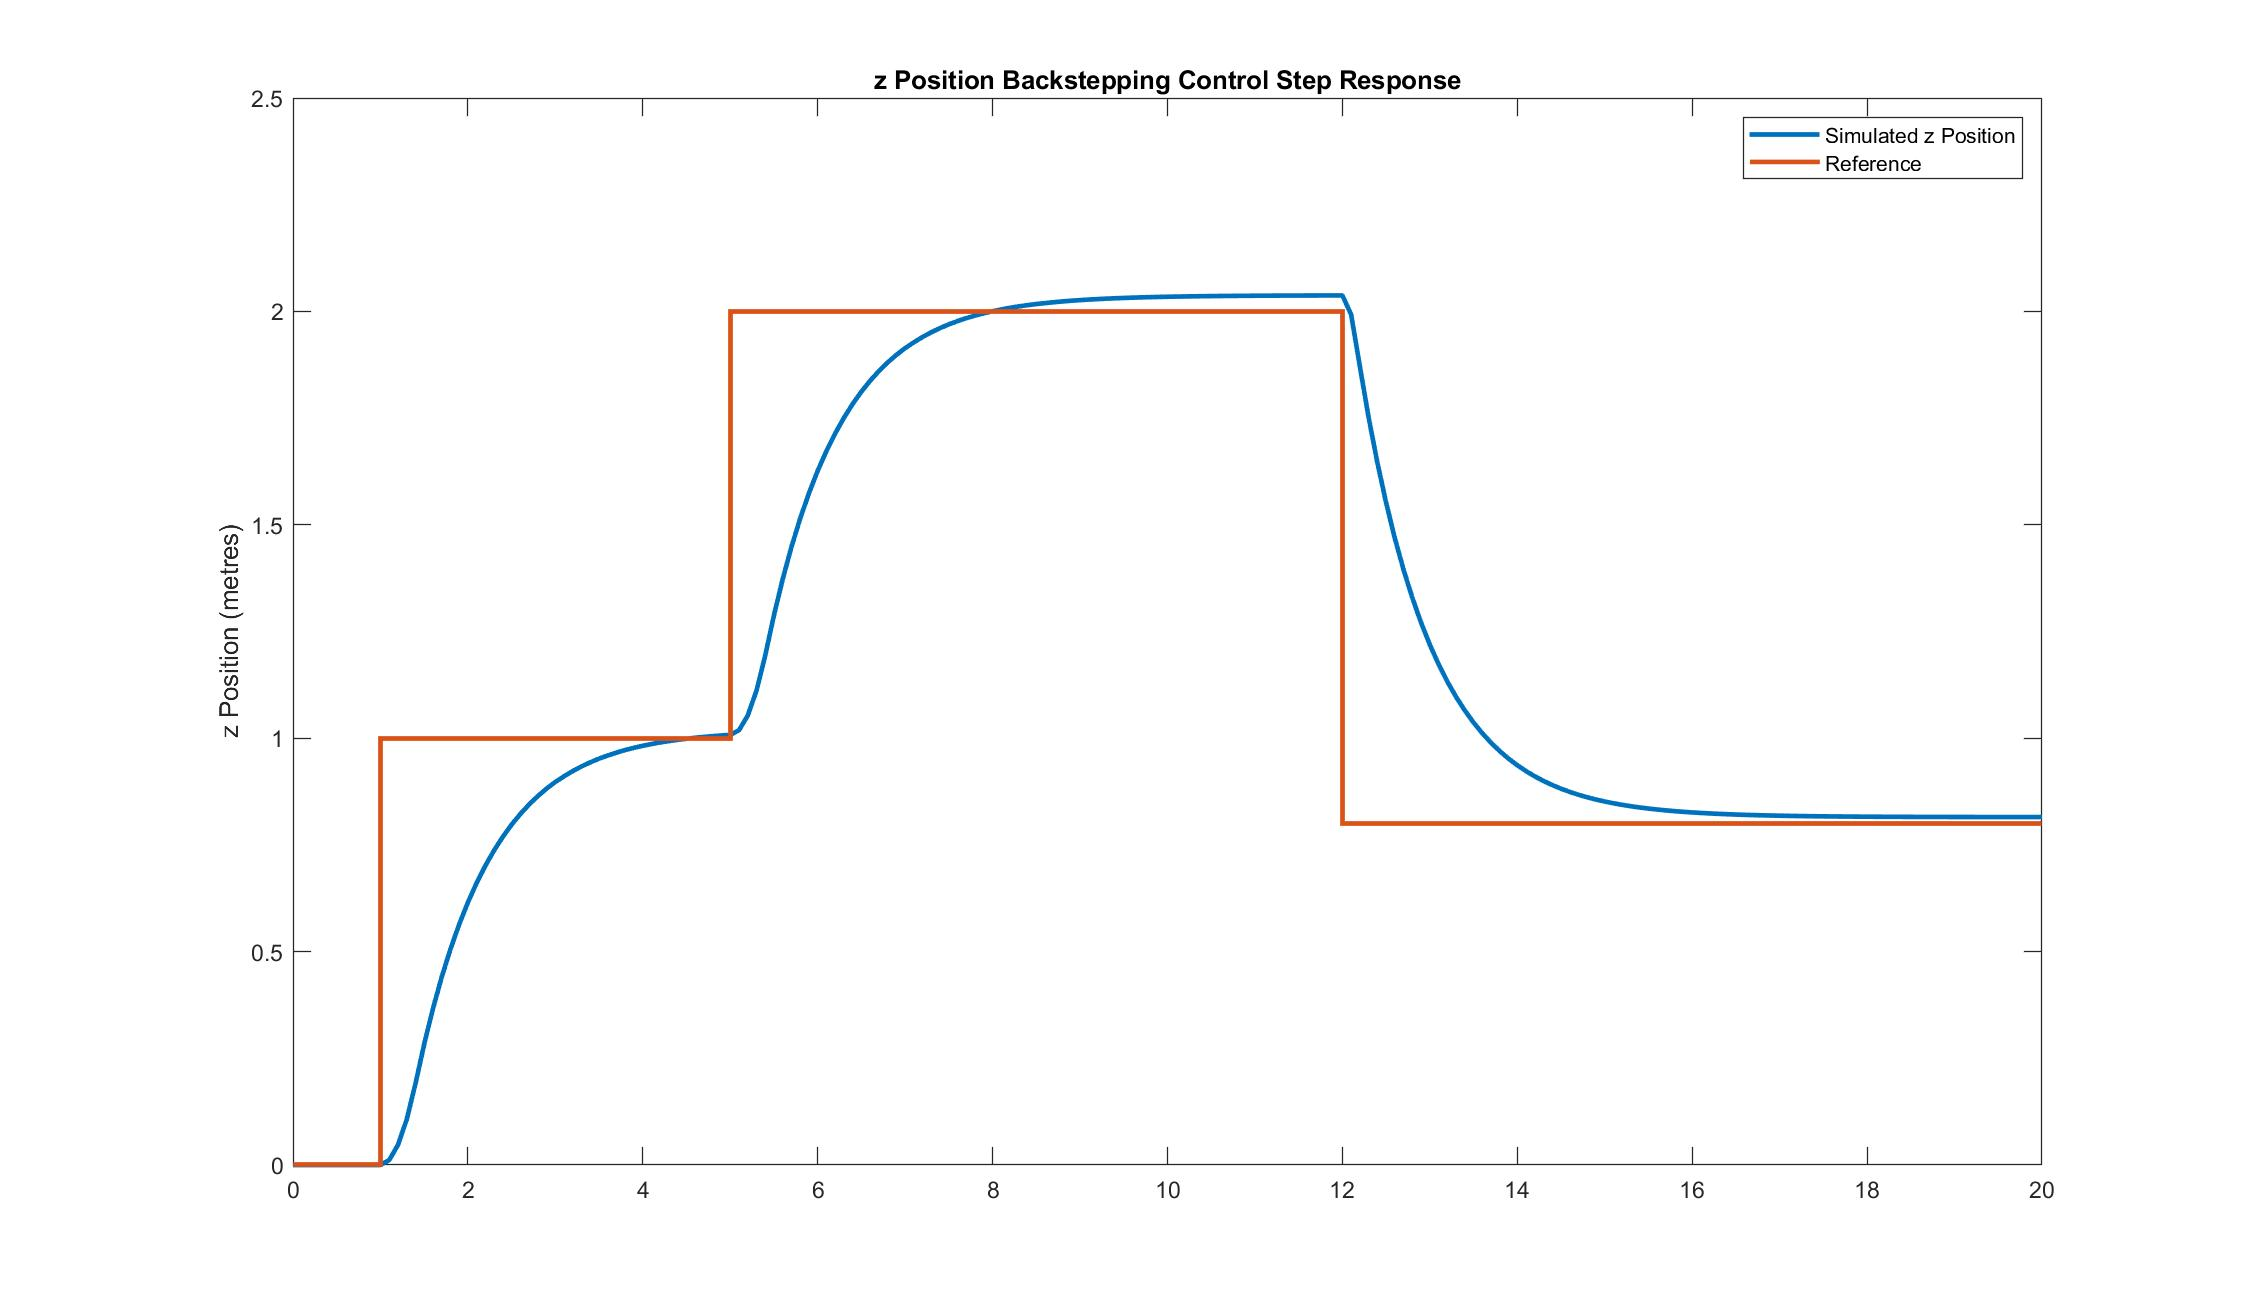
\includegraphics[width=70mm]{/Backstepping_Results/zTracking.jpg}%
	\end{center}
	\caption{Backstepping position and altitude tracking}%
	\label{fig:Backstep_posTrack}%
\end{figure}

\begin{figure}[htb]
\begin{center}
	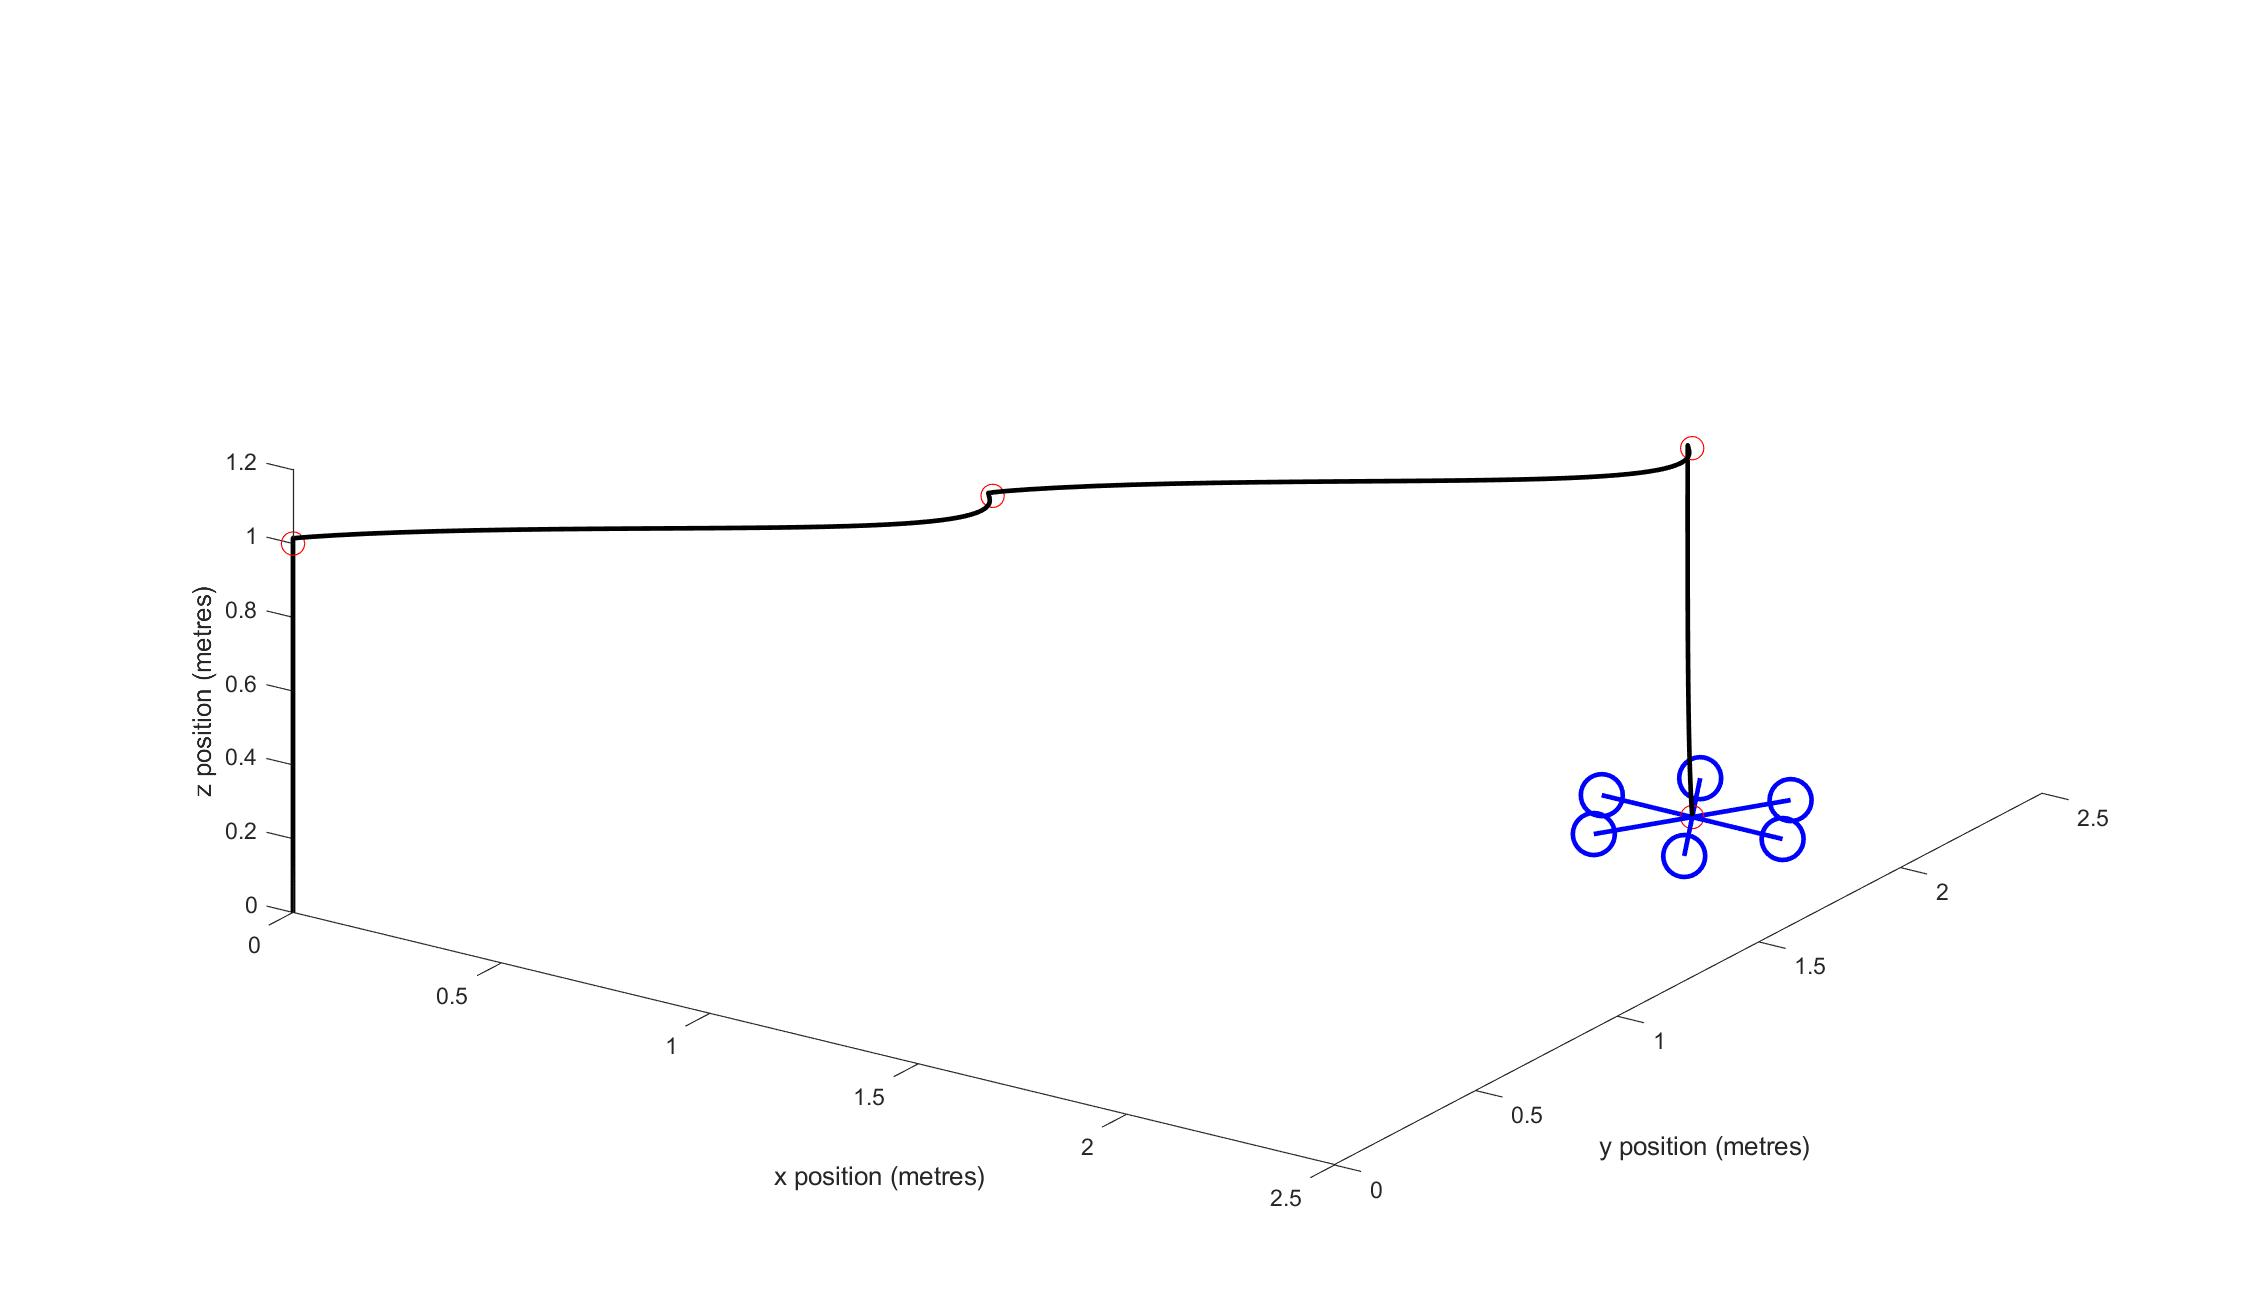
\includegraphics[width=\columnwidth]{/Backstepping_Results/3D_Path_Waypoints3.jpg}%
	\end{center}
	\caption{Backstepping 3D waypoint tracking}%
	\label{fig:Backstep_path}%
\end{figure}

\FloatBarrier
\section{Backstepping with Integral Action}\label{section:IntBack}
As an extension, to reduce the effects of uncertainties in model parameters it is desirable to include integral action within the controller. This method has been shown to be effective at reducing the effects of uncertainties and increasing the robustness of the controller in both simulation \cite{Jasim2015} and hardware \cite{Bouabdallah2006} implementation.

\subsection{Position Control}

%% NEED TO MAKE MOST OF THESE SYMBOLS BOLD TO REPRESENT VECTORS/MATRICES
This controller will use the angle controllers developed in the previous section, only the position controllers will be adjusted to include integral action. This controller will also be derived by considering the position vector rather than individual components.

Consider the position and velocity error vectors: 
\begin{equation}\label{eqn:ErrorVectors}
\begin{split}
\textbf{\textit{e}}_{p}&=\textbf{\textit{p}}_{d}-\textbf{\textit{p}}=\begin{bmatrix}
x_{d}-x \\ y_{d}-y\\ z_{d}-z
\end{bmatrix}\\
\textbf{\textit{e}}_{v}&=\textbf{\textit{v}}_d-\dot{\textbf{\textit{p}}}=\begin{bmatrix}
v_{d,x}-\dot{x} \\ v_{d,y}-\dot{y} \\ v_{d,z}-\dot{z}
\end{bmatrix}\\
\end{split}
\end{equation}

where $v_{d,x}$, $v_{d,x}$ and $v_{d,x}$ are virtual controls representing the desired translational velocities.

Choose a candidate Lyapunov function including an integral term:
\begin{equation}
\textbf{\textit{V}}=\frac{1}{2}\left(\textbf{\textit{e}}_{p}^{T}\textbf{\textit{e}}_{p}+\textbf{\textit{e}}_{v}^{T}\textbf{\textit{e}}_{v}+\textbf{\textit{k}}\Gamma^{T}\Gamma\right)
\end{equation}
where $\Gamma=\int^{t}_{0} e_{p}(\gamma) d\gamma$ and $\textbf{\textit{k}}$ is a diagonal 3x3 matrix of non-negative constants.
Taking the time derivative gives:
\begin{equation}\label{eqn:IntBackCLFder1}
\dot{\textbf{\textit{V}}}=\textbf{\textit{e}}_{p}^{T}\dot{\textbf{\textit{e}}}_{p}+\textbf{\textit{e}}_{v}^{T}\dot{\textbf{\textit{e}}}_{v}+\textbf{\textit{k}}\Gamma^{T}\dot{\Gamma}
\end{equation}
Now choose $\dot{\textbf{\textit{V}}}$ such that it is negative definite:
\begin{equation}\label{eqn:IntBackCLFder2}
\dot{\textbf{\textit{V}}}=-\textbf{\textit{ce}}_{p}^{T}\textbf{\textit{e}}_{p}-\kappa \textbf{\textit{e}}_{v}^{T}\textbf{\textit{e}}_{v}
\end{equation}
where \textbf{\textit{c}} and $\kappa$ represent diagonal 3x3 matrices of non-negative constants.

Now consider the derivative terms:
\begin{equation}\label{eqn:IntBackErrDer}
\begin{split}
\dot{\textbf{\textit{e}}}_{p}&=\dot{\textbf{\textit{p}}}_{d}-\dot{\textbf{\textit{p}}}\\
&=\dot{\textbf{\textit{p}}}_{d}-\textbf{\textit{v}}\\\\
\dot{\textbf{\textit{e}}}_{v}&=\dot{\textbf{\textit{v}}}_{d}-\ddot{\textbf{\textit{p}}}\\\\
\dot{\Gamma}&=\textbf{\textit{e}}_{p}
\end{split}
\end{equation}

The virtual control $\textbf{\textit{v}}_{d}$ is then chosen such that \eqref{eqn:IntBackCLFder1} satisfies \eqref{eqn:IntBackCLFder2}:

\begin{equation*}
\textbf{\textit{v}}_{d}= \dot{\textbf{\textit{p}}}_{d}+\textbf{\textit{ce}}_{p}+\textbf{\textit{k}}\Gamma
\end{equation*}
Substituting into the expression for $\textbf{\textit{e}}_{v}$ in \eqref{eqn:ErrorVectors} gives:

\begin{equation}\label{eqn:e_p1}
\begin{split}
\textbf{\textit{e}}_{v}&=\mathbf{\dot{\textbf{\textit{p}}}}_{d}+\textbf{\textit{ce}}_{p}+\textbf{\textit{k}}\Gamma - \dot{\textbf{\textit{p}}}\\
\textbf{\textit{e}}_{v}-\textbf{\textit{ce}}_{p}-\textbf{\textit{k}}\Gamma&=\dot{\textbf{\textit{p}}}_{d}- \dot{\textbf{\textit{p}}}\\
\dot{\textbf{\textit{e}}_{p}}&=\textbf{\textit{e}}_{v}-\textbf{\textit{ce}}_{p}-\textbf{\textit{k}}\Gamma
\end{split}
\end{equation}
 

Taking the time derivative of $\textbf{\textit{e}}_{v}$ gives:
\begin{equation}\label{eqn:dot_e_v1}
\begin{split}
\dot{\textbf{\textit{e}}}_{v}&=\ddot{\textbf{\textit{p}}}_{d}+\textbf{\textit{c}}\dot{\textbf{\textit{e}}}_{p}+\textbf{\textit{k}} \textbf{\textit{e}}_{p} - \ddot{\textbf{\textit{p}}}\\
\dot{\textbf{\textit{e}}}_{v}&=\ddot{\textbf{\textit{p}}}_{d}+\textbf{\textit{c}}(\textbf{\textit{e}}_{v}-\textbf{\textit{ce}}_{p}-\textbf{\textit{k}}\Gamma)+\textbf{\textit{k}} \textbf{\textit{e}}_{p} - \ddot{\textbf{\textit{p}}}\\
\dot{\textbf{\textit{e}}}_{v}&=\ddot{\textbf{\textit{p}}}_{d}+\textbf{\textit{ce}}_{v}-\textbf{\textit{c}}^{2}\textbf{\textit{e}}_{p}-\textbf{\textit{ck}}\Gamma+\textbf{\textit{k}} \textbf{\textit{e}}_{p} - \ddot{\textbf{\textit{p}}}\\
\end{split}
\end{equation} 

Note that an expression for the second derivative of translational position ($\ddot{\textbf{\textit{p}}}$) is given in Section \ref{section:AddTransMotion}, \eqref{eqn:additionalState2}. Also note that in order to satisfy \eqref{eqn:IntBackCLFder2}, $\dot{\textbf{\textit{e}}}_{v}$ is chosen as:
\begin{equation}\label{eqn:dot_e_v2}
\dot{\textbf{\textit{e}}}_{v}=-\kappa \textbf{\textit{e}}_{v} - \textbf{\textit{e}}_{p}
\end{equation}
Finally, equating \eqref{eqn:dot_e_v1} with \eqref{eqn:dot_e_v2} allows the control laws to be derived:
\begin{equation}\label{eqn:dot_e_v3}
\begin{split}
-\kappa \textbf{\textit{e}}_{v} - \textbf{\textit{e}}_{p}&=\ddot{\textbf{\textit{p}}}_{d}+\textbf{\textit{ce}}_{v}-\textbf{\textit{c}}^{2}\textbf{\textit{e}}_{p}-\textbf{\textit{ck}}\Gamma+\textbf{\textit{ke}}_{p} - \ddot{\textbf{\textit{p}}}\\
\ddot{\textbf{\textit{p}}}&=\ddot{\textbf{\textit{p}}}_{d}+\textbf{\textit{ce}}_{v}-\textbf{\textit{c}}^{2}\textbf{\textit{e}}_{p}-\textbf{\textit{ck}}\Gamma+\textbf{\textit{ke}}_{p} +\kappa \textbf{\textit{e}}_{v} + \textbf{\textit{e}}_{p}\\
\ddot{\textbf{\textit{p}}}&=\ddot{\textbf{\textit{p}}}_{d}+(1+\textbf{\textit{k}}-\textbf{\textit{c}}^{2})\textbf{\textit{e}}_{p}+(\textbf{\textit{c}}+\kappa)\textbf{\textit{e}}_{v}-\textbf{\textit{ck}}\Gamma
\end{split}
\end{equation}

The control laws are then derived using $\theta_{d}$, $\phi_{d}$ and $F_{T}$ as the control inputs.

 \begin{equation}\label{eqn:IntBackContLaws}
\begin{split}
\theta_{d}&=sin^{-1}\left(\frac{-\frac{m}{F_{T}}[\ddot{x}_{d}+(1+k_{1}-c_{1}^{2})e_{x}+(c_{1}+\kappa_{1})e_{v,x}-c_{1}k_{1}\Gamma_{1}]-sin(\phi)sin(\psi)}{cos(\phi)cos(\psi)}\right)\\
\phi_{d}&=sin^{-1}\left(\frac{\frac{m}{F_{T}}[\ddot{y}_{d}+(1+k_{2}-c_{2}^{2})e_{y}+(c_{2}+\kappa_{2})e_{v,y}-c_{2}k_{2}\Gamma_{2}]+cos(\phi)sin(\theta)sin(\psi)}{cos(\psi)}\right)\\
F_{T}&=\frac{m(\ddot{z}_{d}(1+k_{3}-c_{3}^{2})e_{z}+(c+\kappa_{3})e_{v,z}-c_{3}k_{3}\Gamma_{3}+g)}{cos(\phi)cos(\theta)}
\end{split}
\end{equation}




\FloatBarrier
\subsection{Preliminary Results}
The position and altitude tracking results are shown in \figref{fig:IntBackPos}. This demonstrates the ability of this control system to track positional commands with zero steady state error. This system is also more robust to model uncertainties. The angle controllers are unchanged from the previous section, thus the angle stabilising result is omitted in this section. 

\begin{figure}[htb]
\begin{center}
	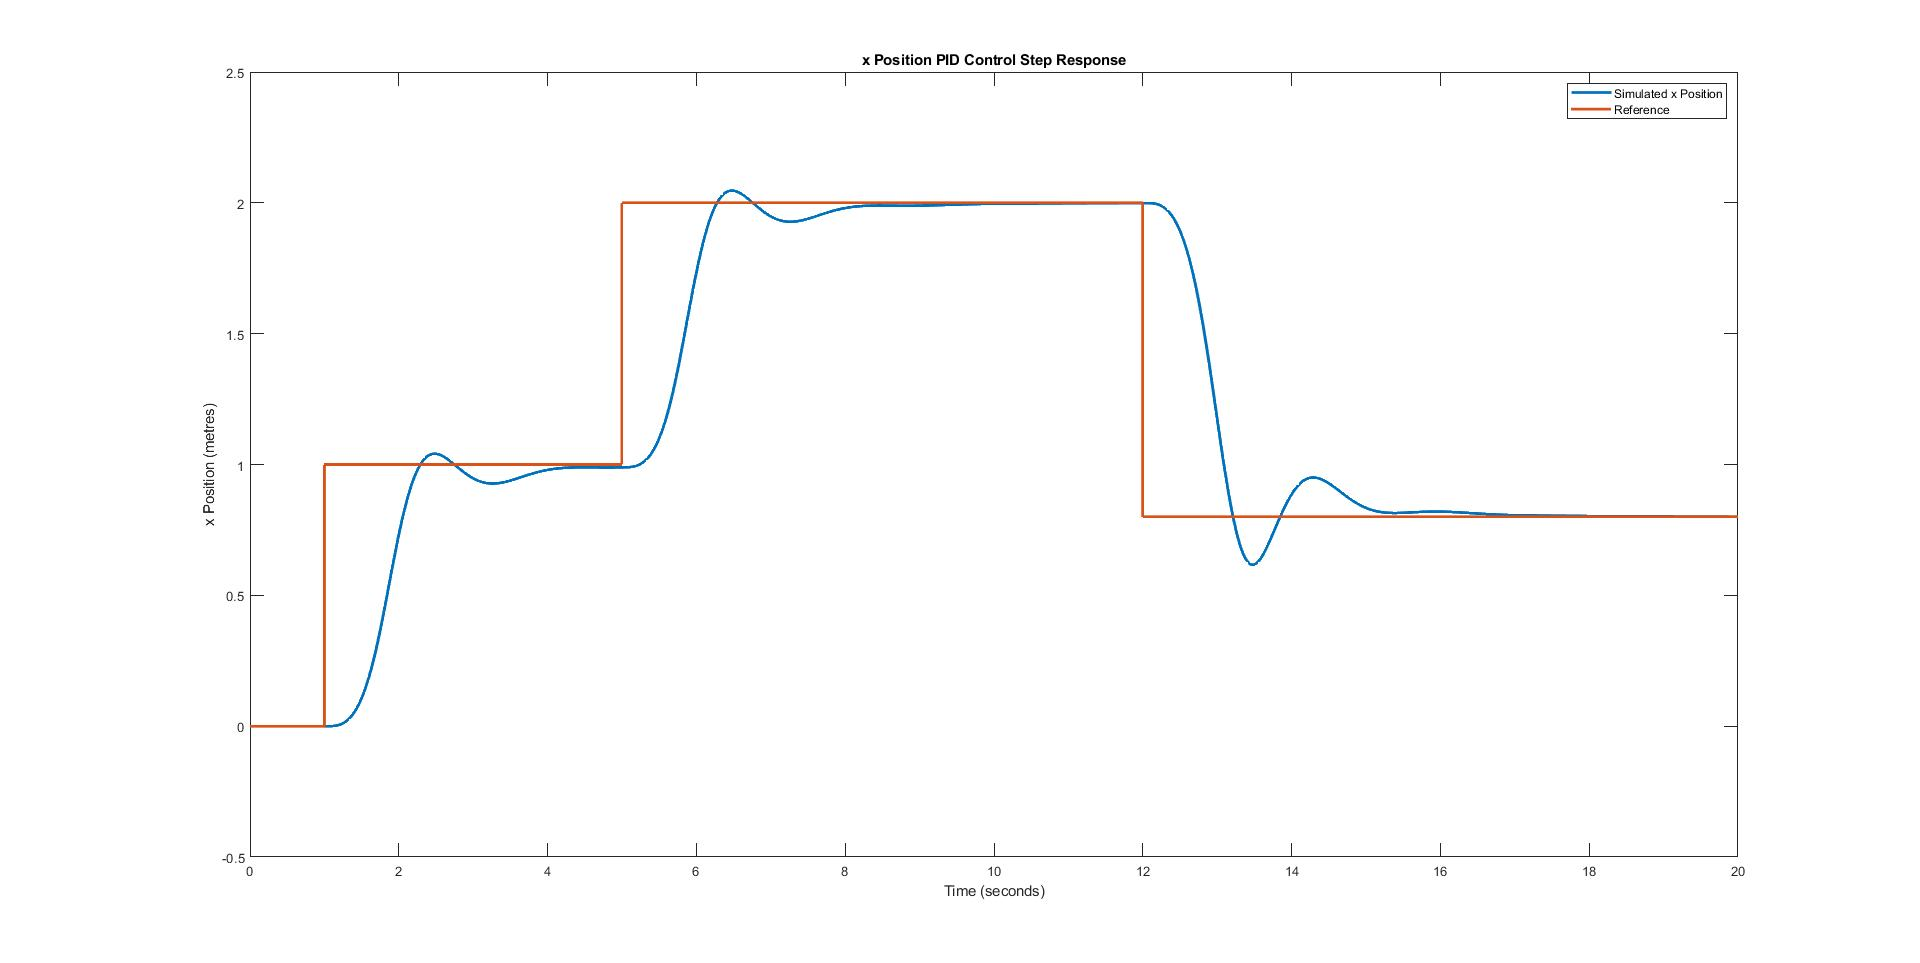
\includegraphics[width=70mm]{/Integral_Backstepping_Results/xTracking_Steps.jpg}%
	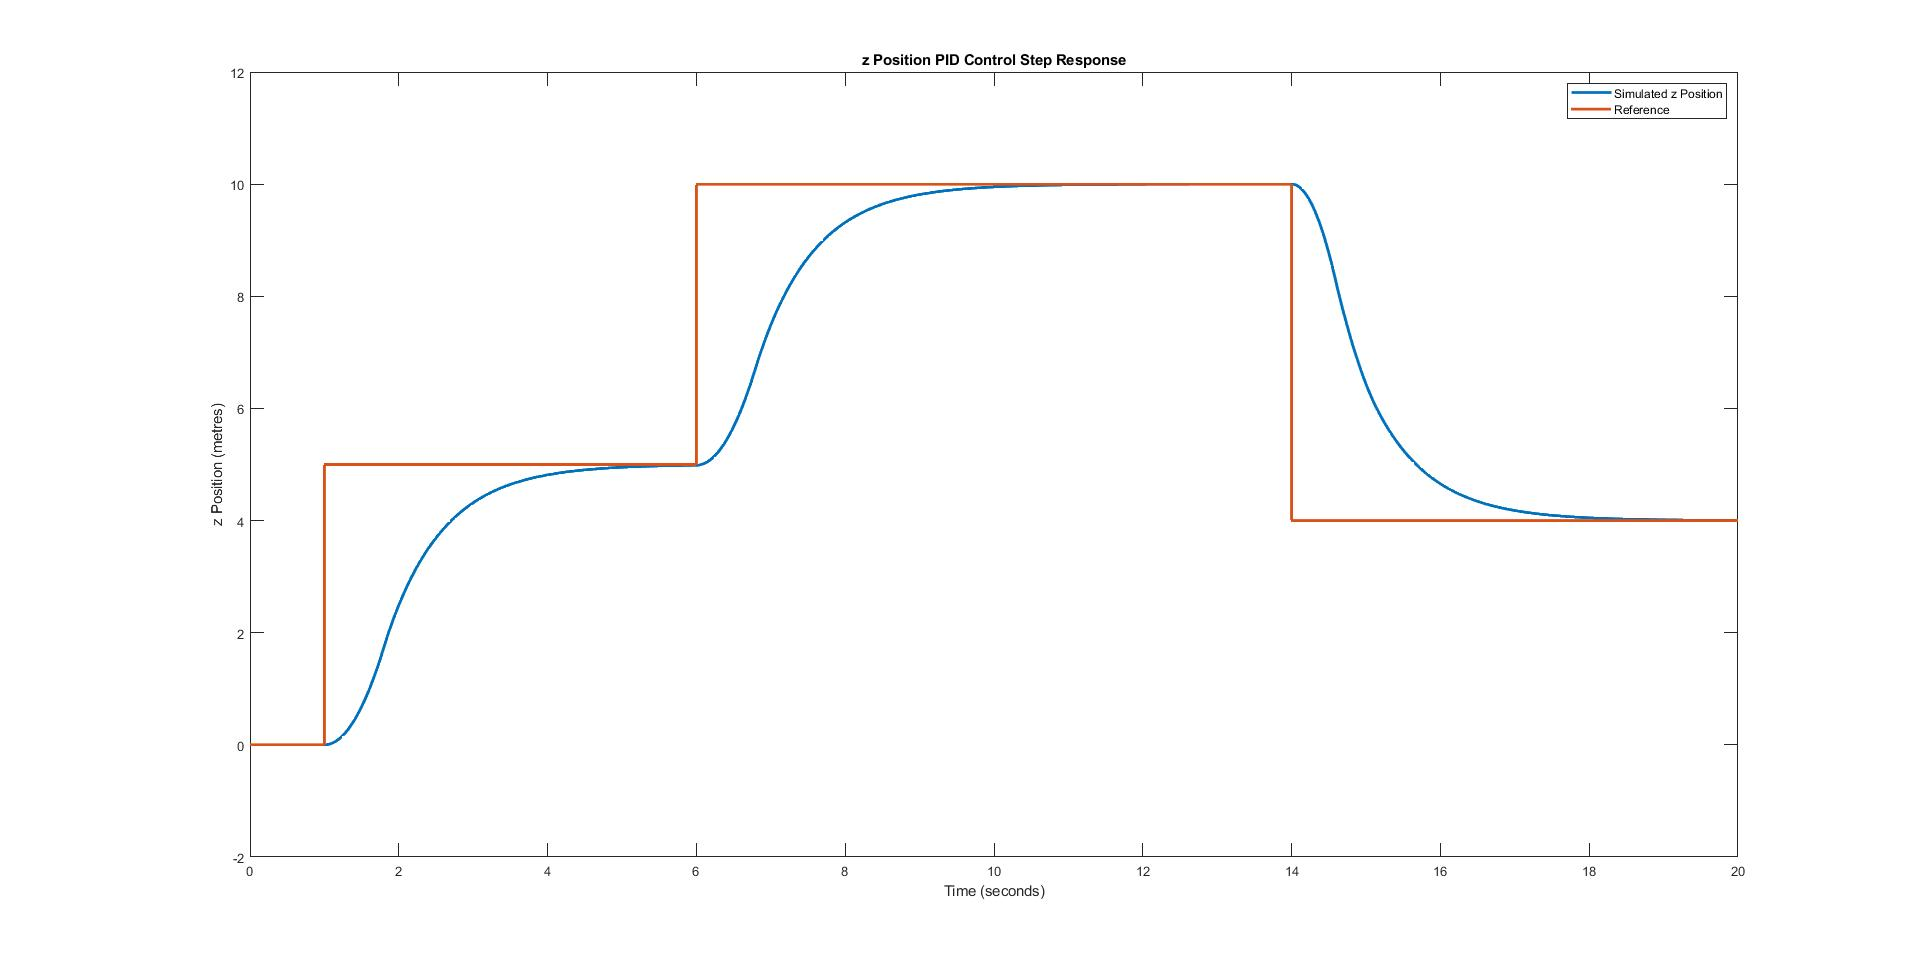
\includegraphics[width=70mm]{/Integral_Backstepping_Results/zTracking_Steps.jpg}%
	\end{center}
	\caption{Integral Backstepping position tracking}%
	\label{fig:IntBackPos}%
\end{figure}

A persisting limitation with this control method is its inability to stabilise when presented with a large step input. \figref{fig:IntBackSat} shows the system response to a ten metre step command in the x direction.

\begin{figure}[htb]
\begin{center}
	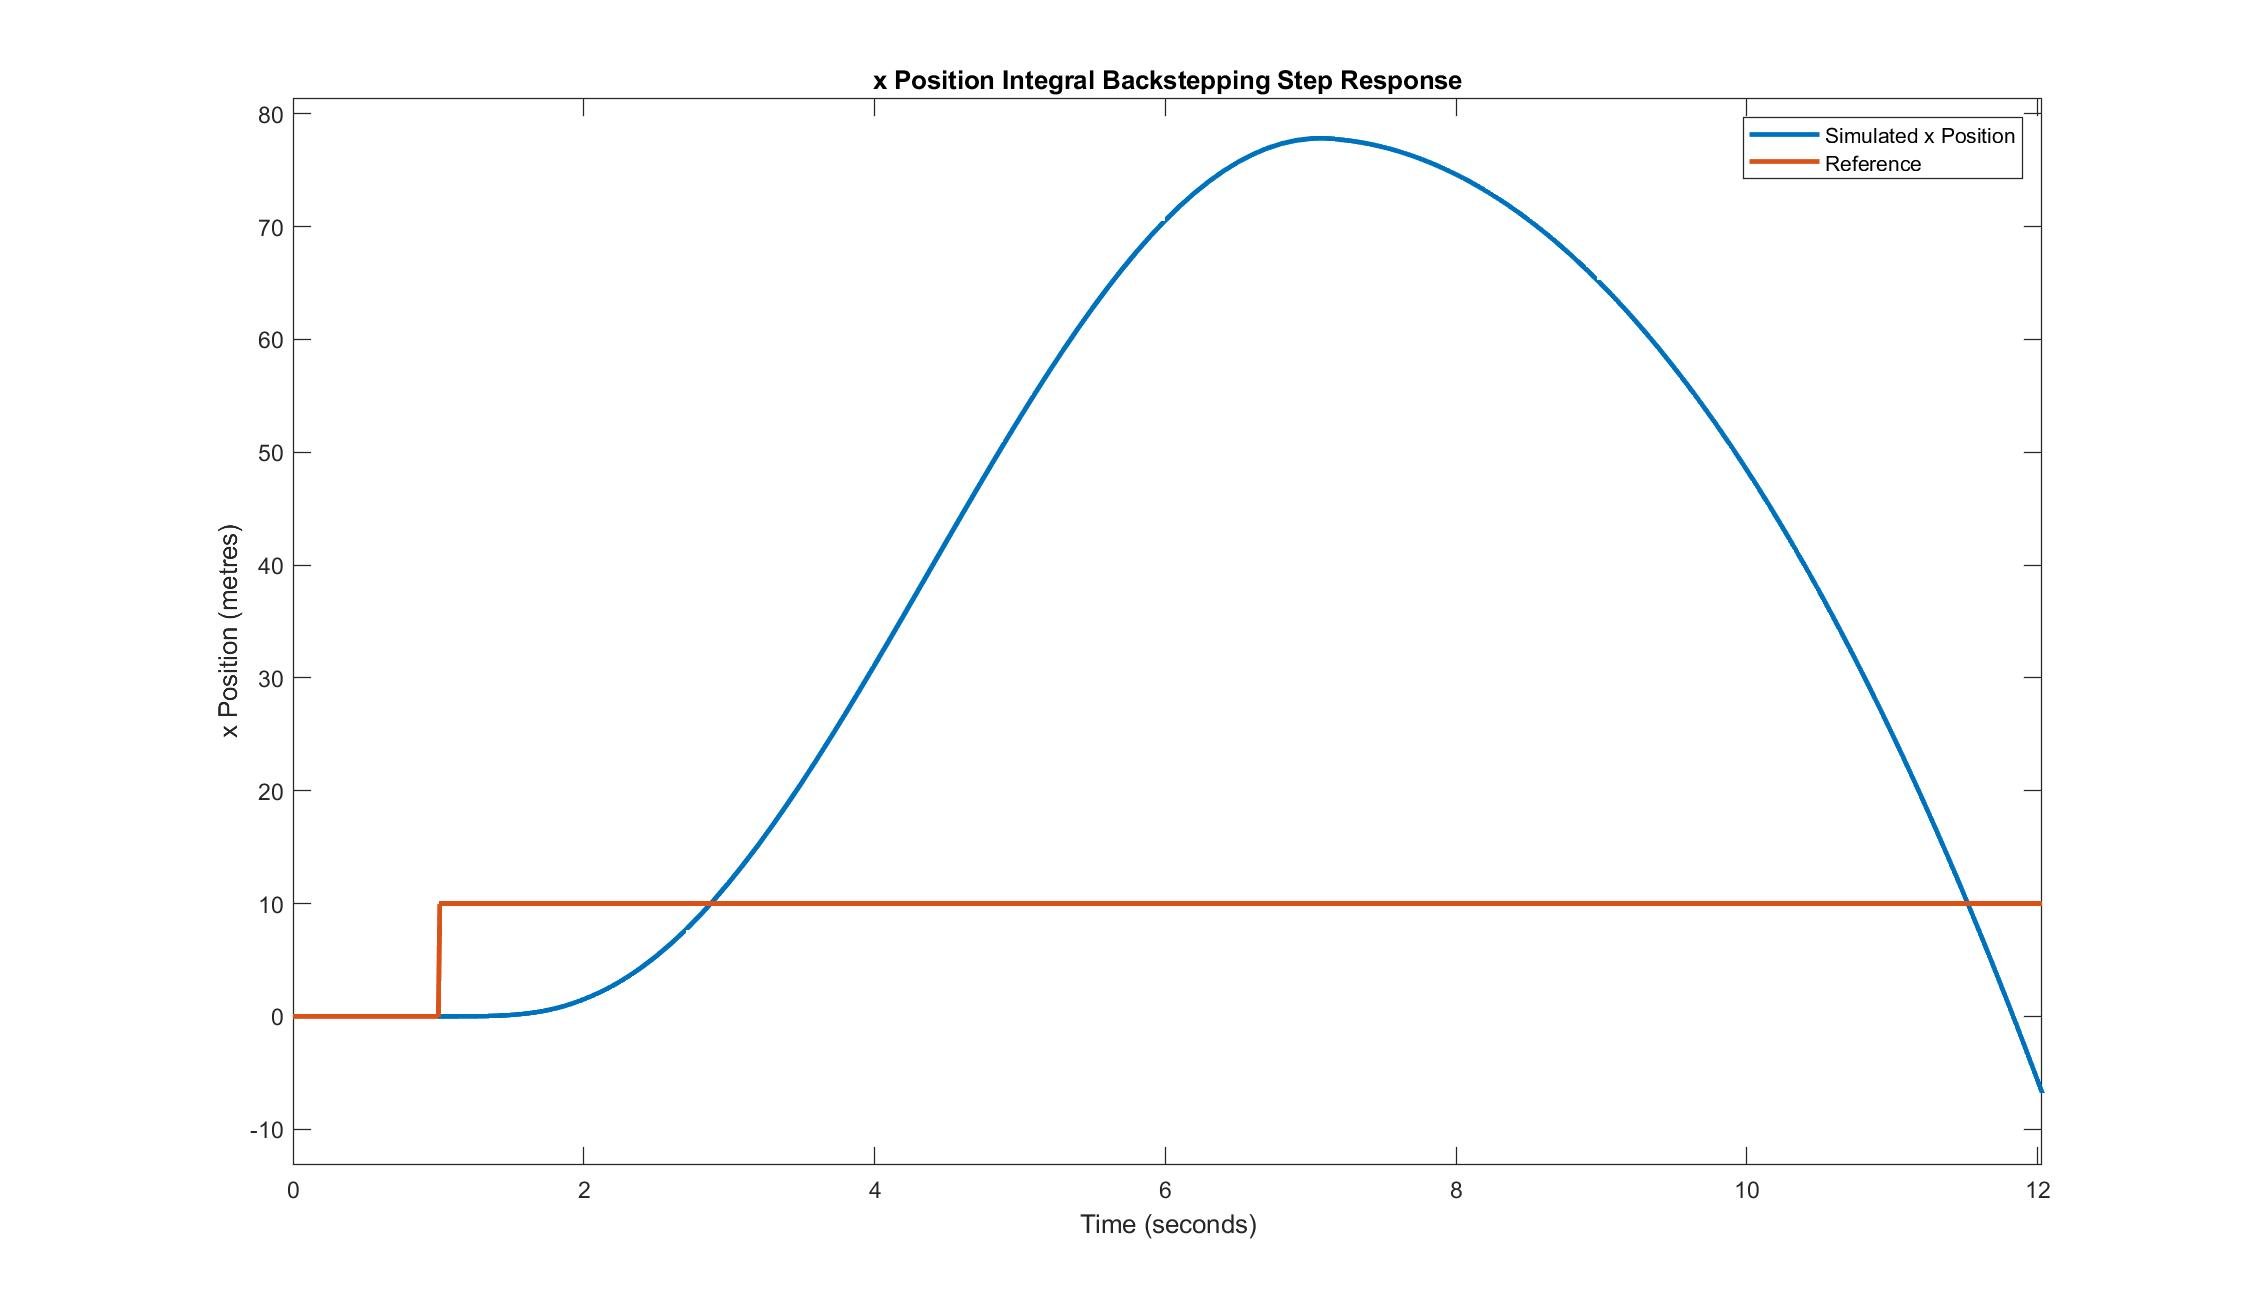
\includegraphics[width=70mm]{/Integral_Backstepping_Results/x_Saturation.jpg}%
	\end{center}
	\caption{Integral backstepping response to a large step input}%
	\label{fig:IntBackSat}%
\end{figure}
\FloatBarrier
\section{Actuator Saturation}
To prevent actuator saturation when large step commands are given, a sigmoid function can be used to limit the effect of position error \cite{Cabecinhas2009}. For this purpose, the sigmoid function is defined as:
\[\sigma(x)=p_{max}\frac{x}{1+|x|}\]

This sigmoid function is used to limit the output of the x and y position controllers prior to the arcsine function. The parameter $p_{max}$ is chosen as 0.77 to limit the desired roll and pitch angles to $\pm50^{\circ}$.
This greatly improves the controllers response to large step inputs, as can be seen by comparing the ten metre step response in \figref{fig:SatStep} with \figref{fig:IntBackSat}.

\begin{figure}[htb]
\begin{center}
	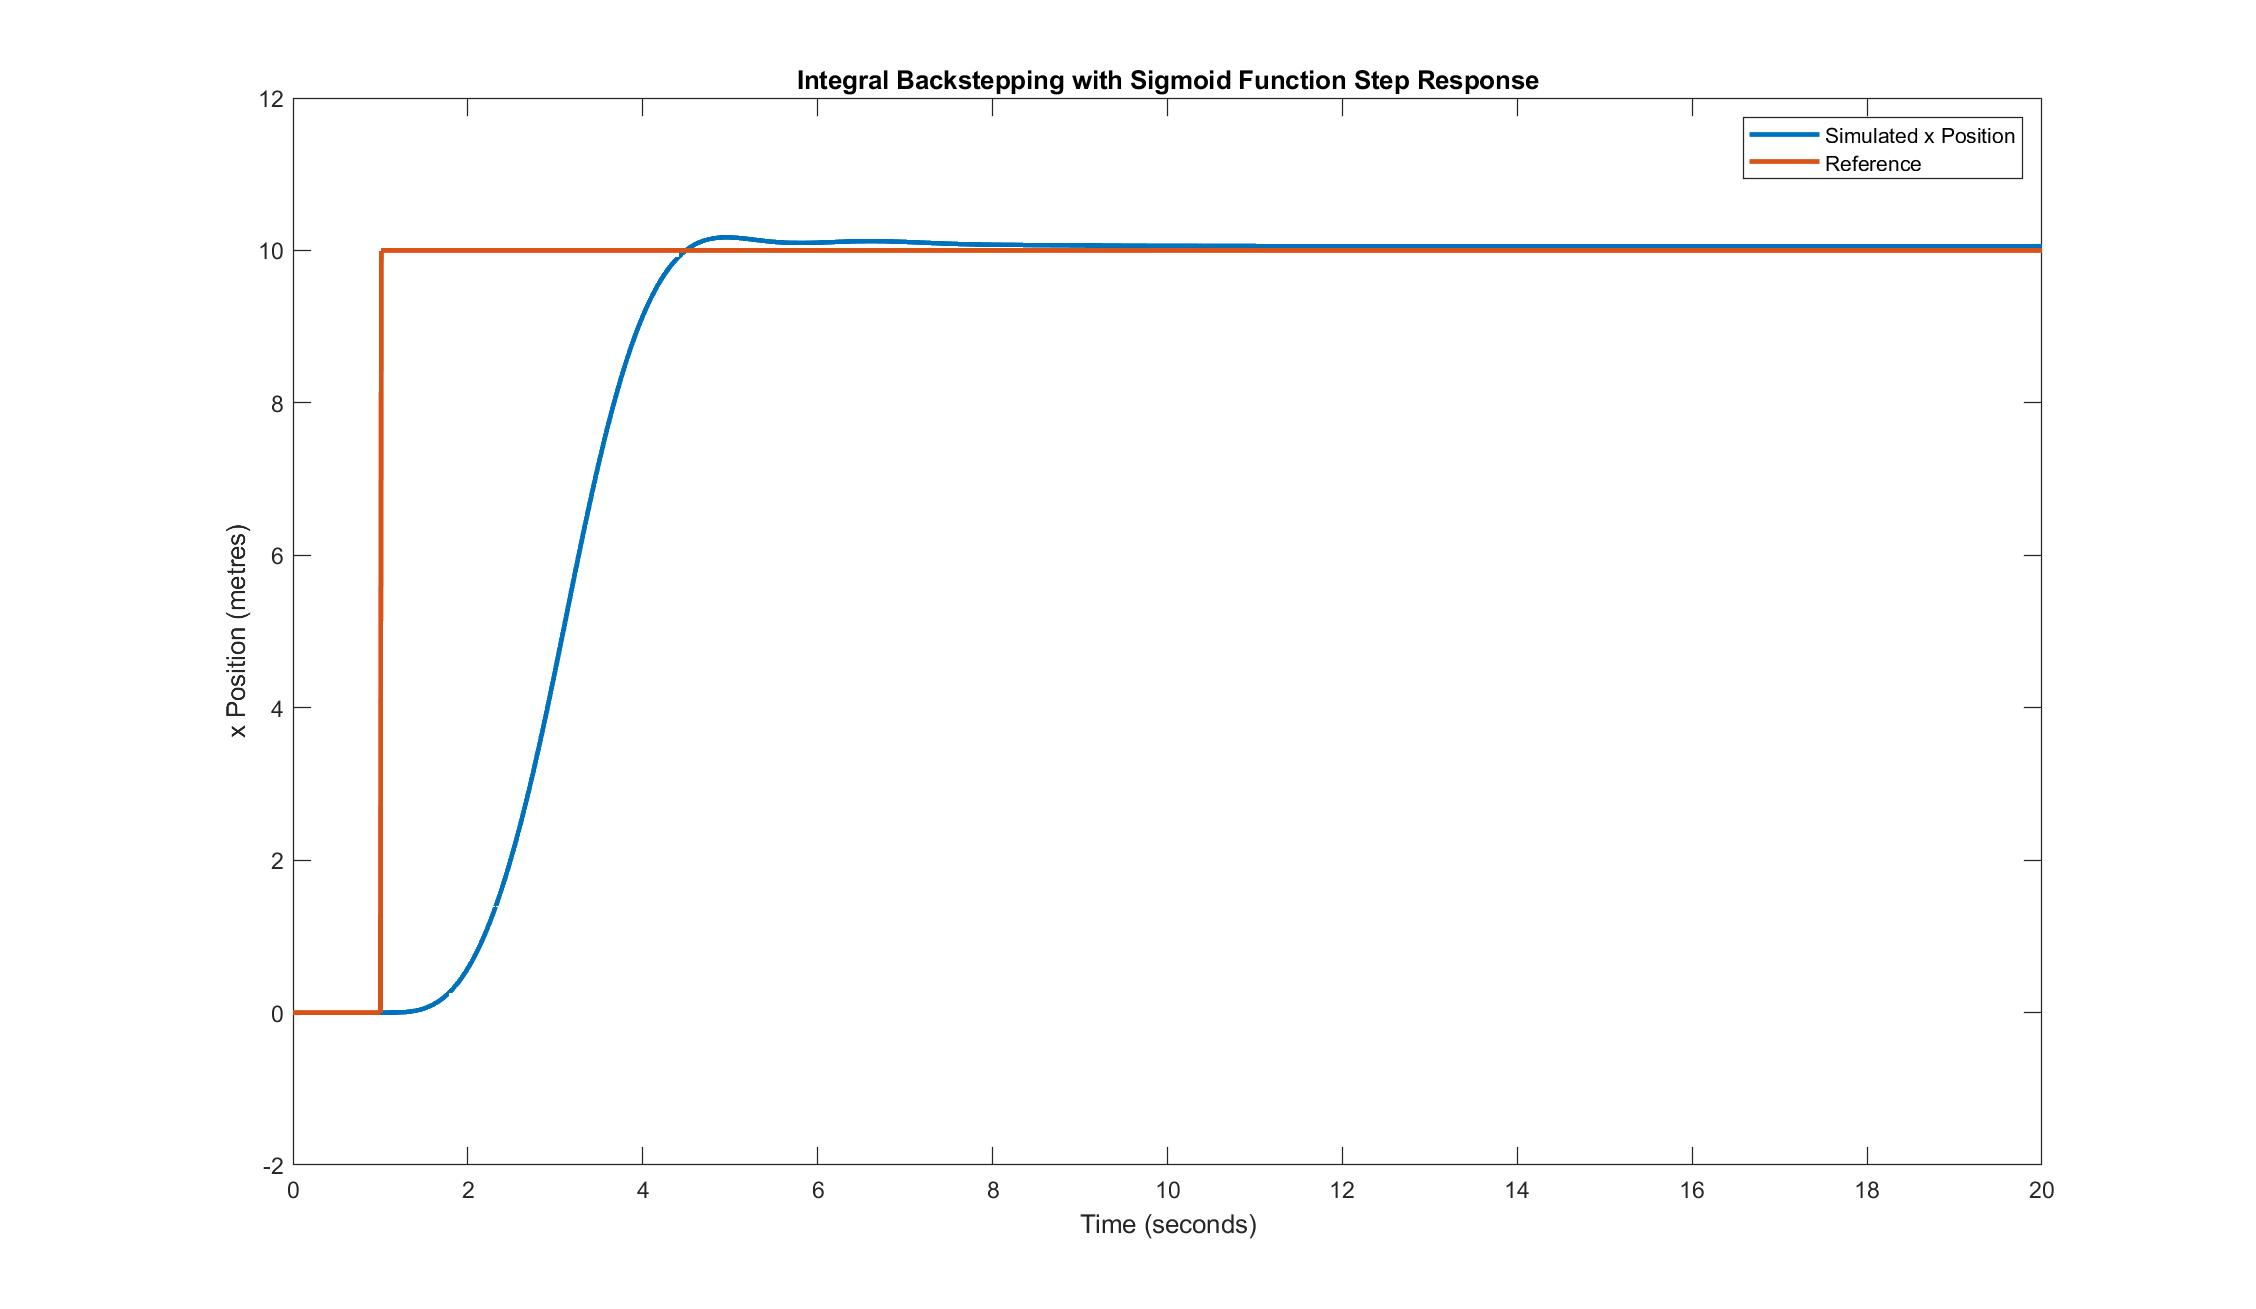
\includegraphics[width=\columnwidth]{/Saturation/xTracking_Step.jpg}%
	\end{center}
	\caption{Integral Backstepping position tracking with sigmoid function}%
	\label{fig:SatStep}%
\end{figure}

\section{Final Control System}
The final control system was developed progressively and documented throughout this chapter. The attitude control laws are based upon backstepping control and are those displayed in \eqref{eqn:BackstepPhiLaw} and \eqref{eqn:BackstepAngleLaws}. The position controllers include the addition of integral action in the backstepping control law, as shown in \eqref{eqn:IntBackContLaws}. The Simulink model for the entire control system and each subsystem is shown in Appendix \ref{section:Simu_Control}.

Again the constant gain values were tuned using the Simulink Design Optimization Package. The final gains that were used for this system are given in Table \ref{table:FinalGains}.
\begin{table}[htb]
\begin{center}
\begin{tabular}{||c|c|c||}
 \hline
 Controller & Gain & Value\\ [0.5ex] 
 \hline\hline
 \multirow{2}{7em}{Roll Angle}& K\textsubscript{1} & 1.65 \\ 
 \cline{2-3}
  &K\textsubscript{2} & 1.65 \\
 \hline
  \multirow{2}{7em}{Pitch Angle}& K\textsubscript{3} & 2.21 \\
 \cline{2-3}
  &K\textsubscript{4} & 2.21 \\
 \hline
 \multirow{2}{7em}{Yaw Angle}& K\textsubscript{5} & 3.11 \\
 \cline{2-3}
 &K\textsubscript{6} & 3.11 \\
 \hline
 \multirow{2}{7em}{x Position}& c\textsubscript{1} & 3.67 \\
 \cline{2-3}
 &k\textsubscript{1} & 0.01 \\
\cline{2-3}
&$\kappa$\textsubscript{1} & 1.57 \\
 \hline
 \multirow{2}{7em}{y Position}& c\textsubscript{2} & 3.92 \\
 \cline{2-3}
 &k\textsubscript{2} & 0.01 \\
\cline{2-3}
&$\kappa$\textsubscript{2} & 1.35 \\
 \hline
 \multirow{2}{7em}{z Position}& c\textsubscript{3} & 2.50 \\
 \cline{2-3}
 &k\textsubscript{3} & 0.01 \\
\cline{2-3}
&$\kappa$\textsubscript{3} & 1.00 \\
 \hline
\end{tabular}
\caption{Final control system gains}
\label{table:FinalGains}
\end{center}
\end{table}

This controller allows the vehicle to follow waypoint commands. The results in \figref{fig:SatWaypoints} show the path of the simulated vehicle as it travels between four waypoints - separated by 5 metres - before returning to its starting position and landing. The total simulated time for this flight was 40 seconds.

\begin{figure}[htb]
\begin{center}
	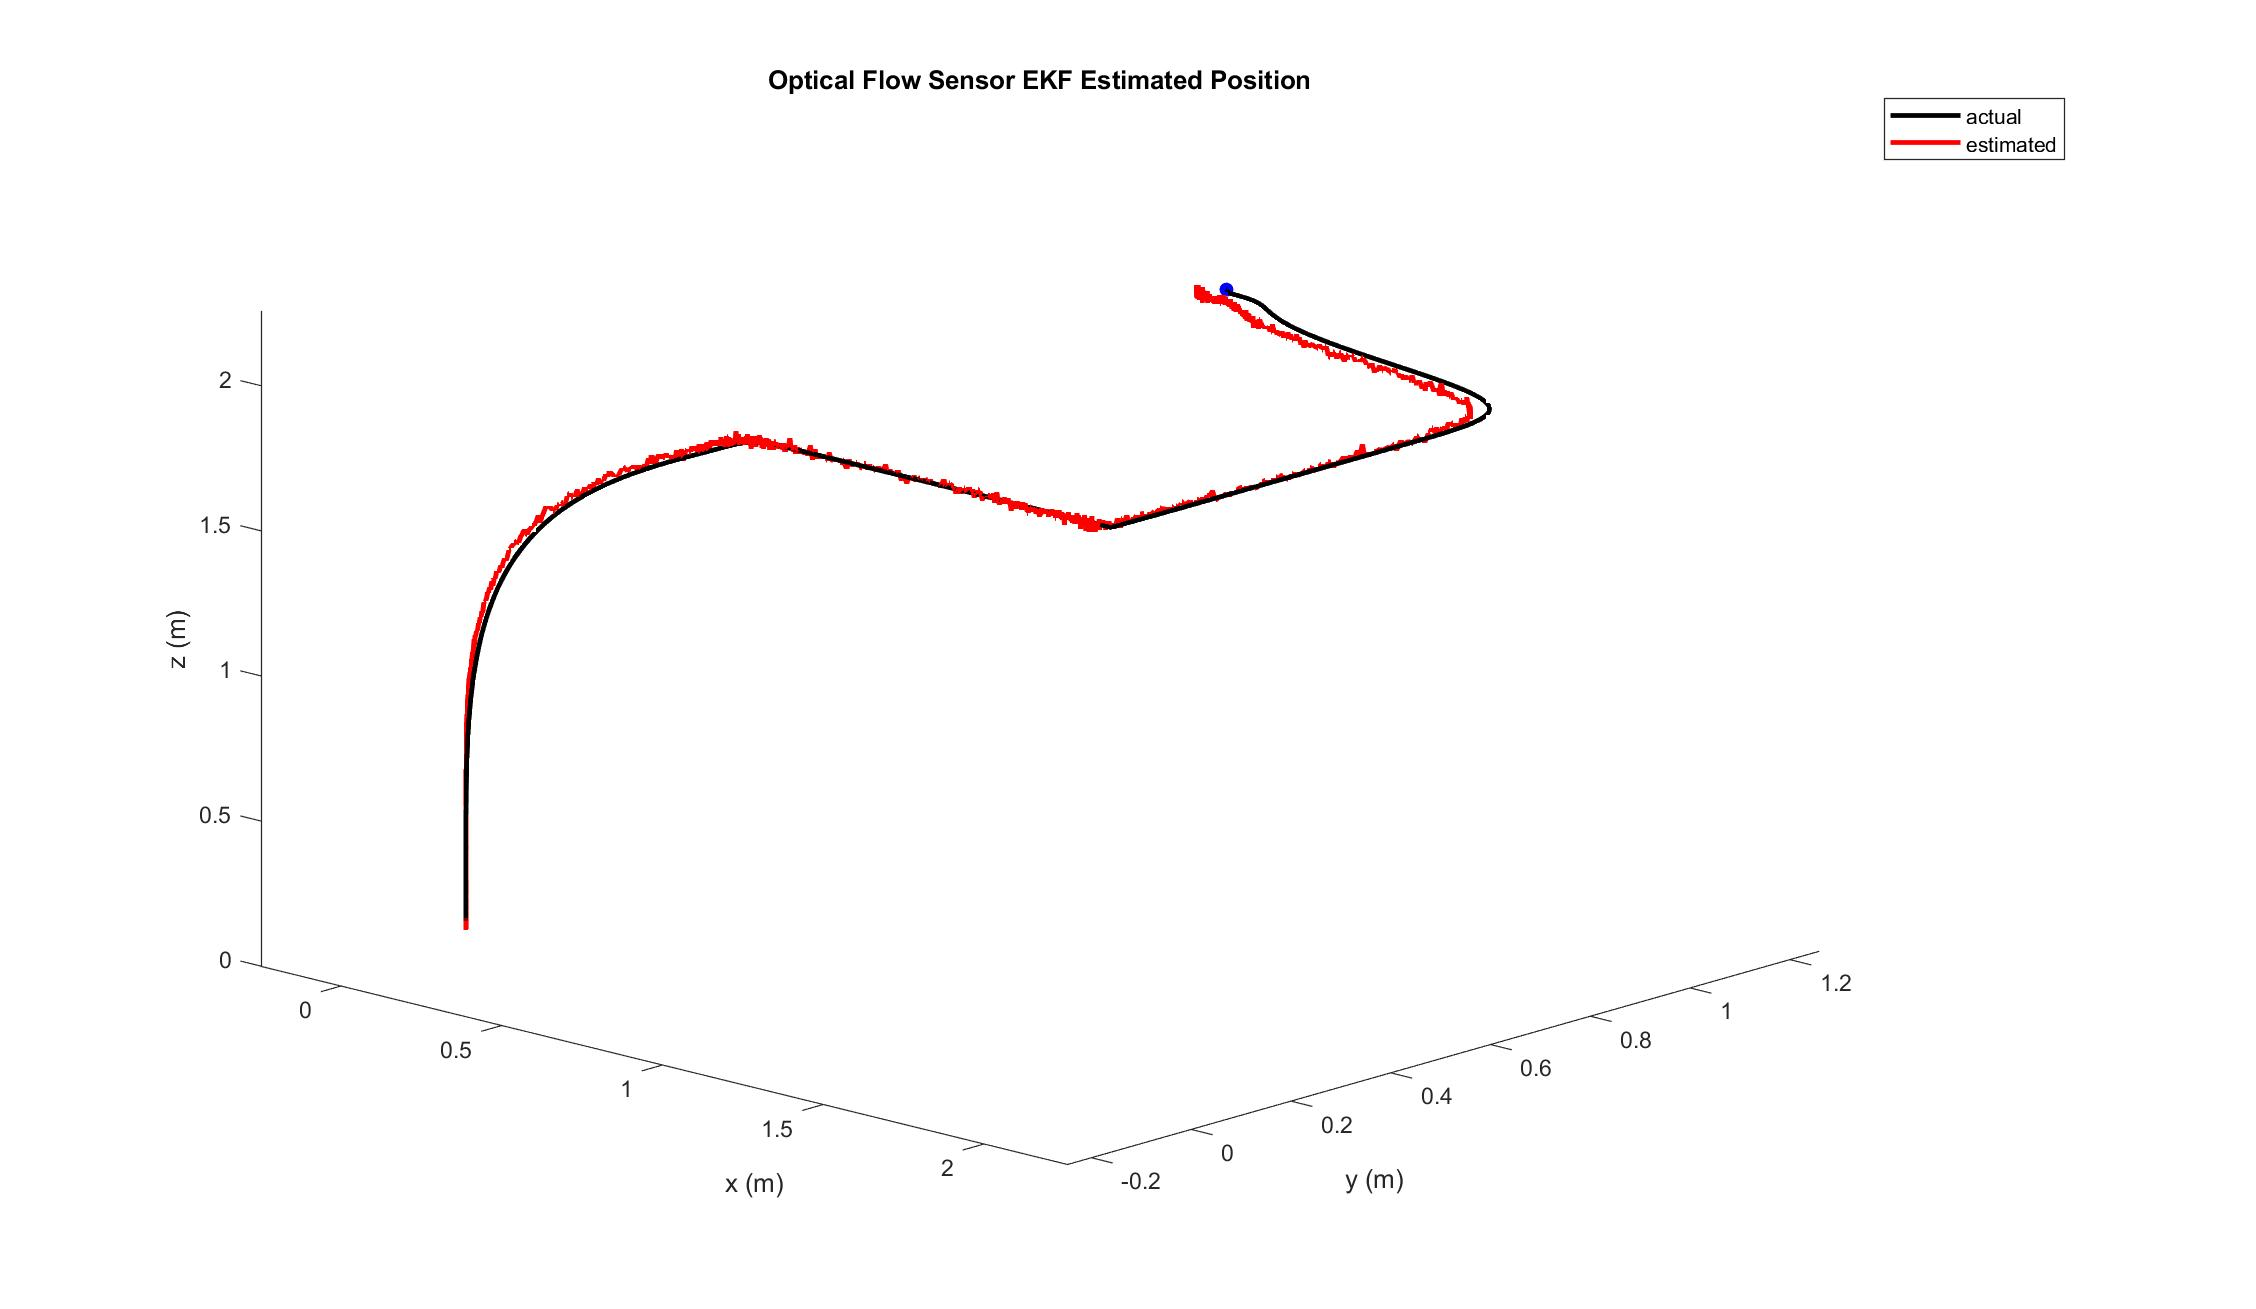
\includegraphics[width=\columnwidth]{/Saturation/Waypoints.jpg}%
	\end{center}
	\caption{Final control system waypoint tracking.}%
	\label{fig:SatWaypoints}%
\end{figure}


To investigate the robustness of this controller, process noise was added to the model to simulate effects which were not previously accounted for e.g. wind. Gaussian noise with zero mean and variance of 0.1 was added to the body frame translational motion (u, v) within the model. The same waypoints were given to the control system, and the resulting flight path is shown in \figref{fig:SatWayNoise}. This demonstrates the ability of the control system to handle both external disturbances and model uncertainties.

\begin{figure}[htb]
\begin{center}
	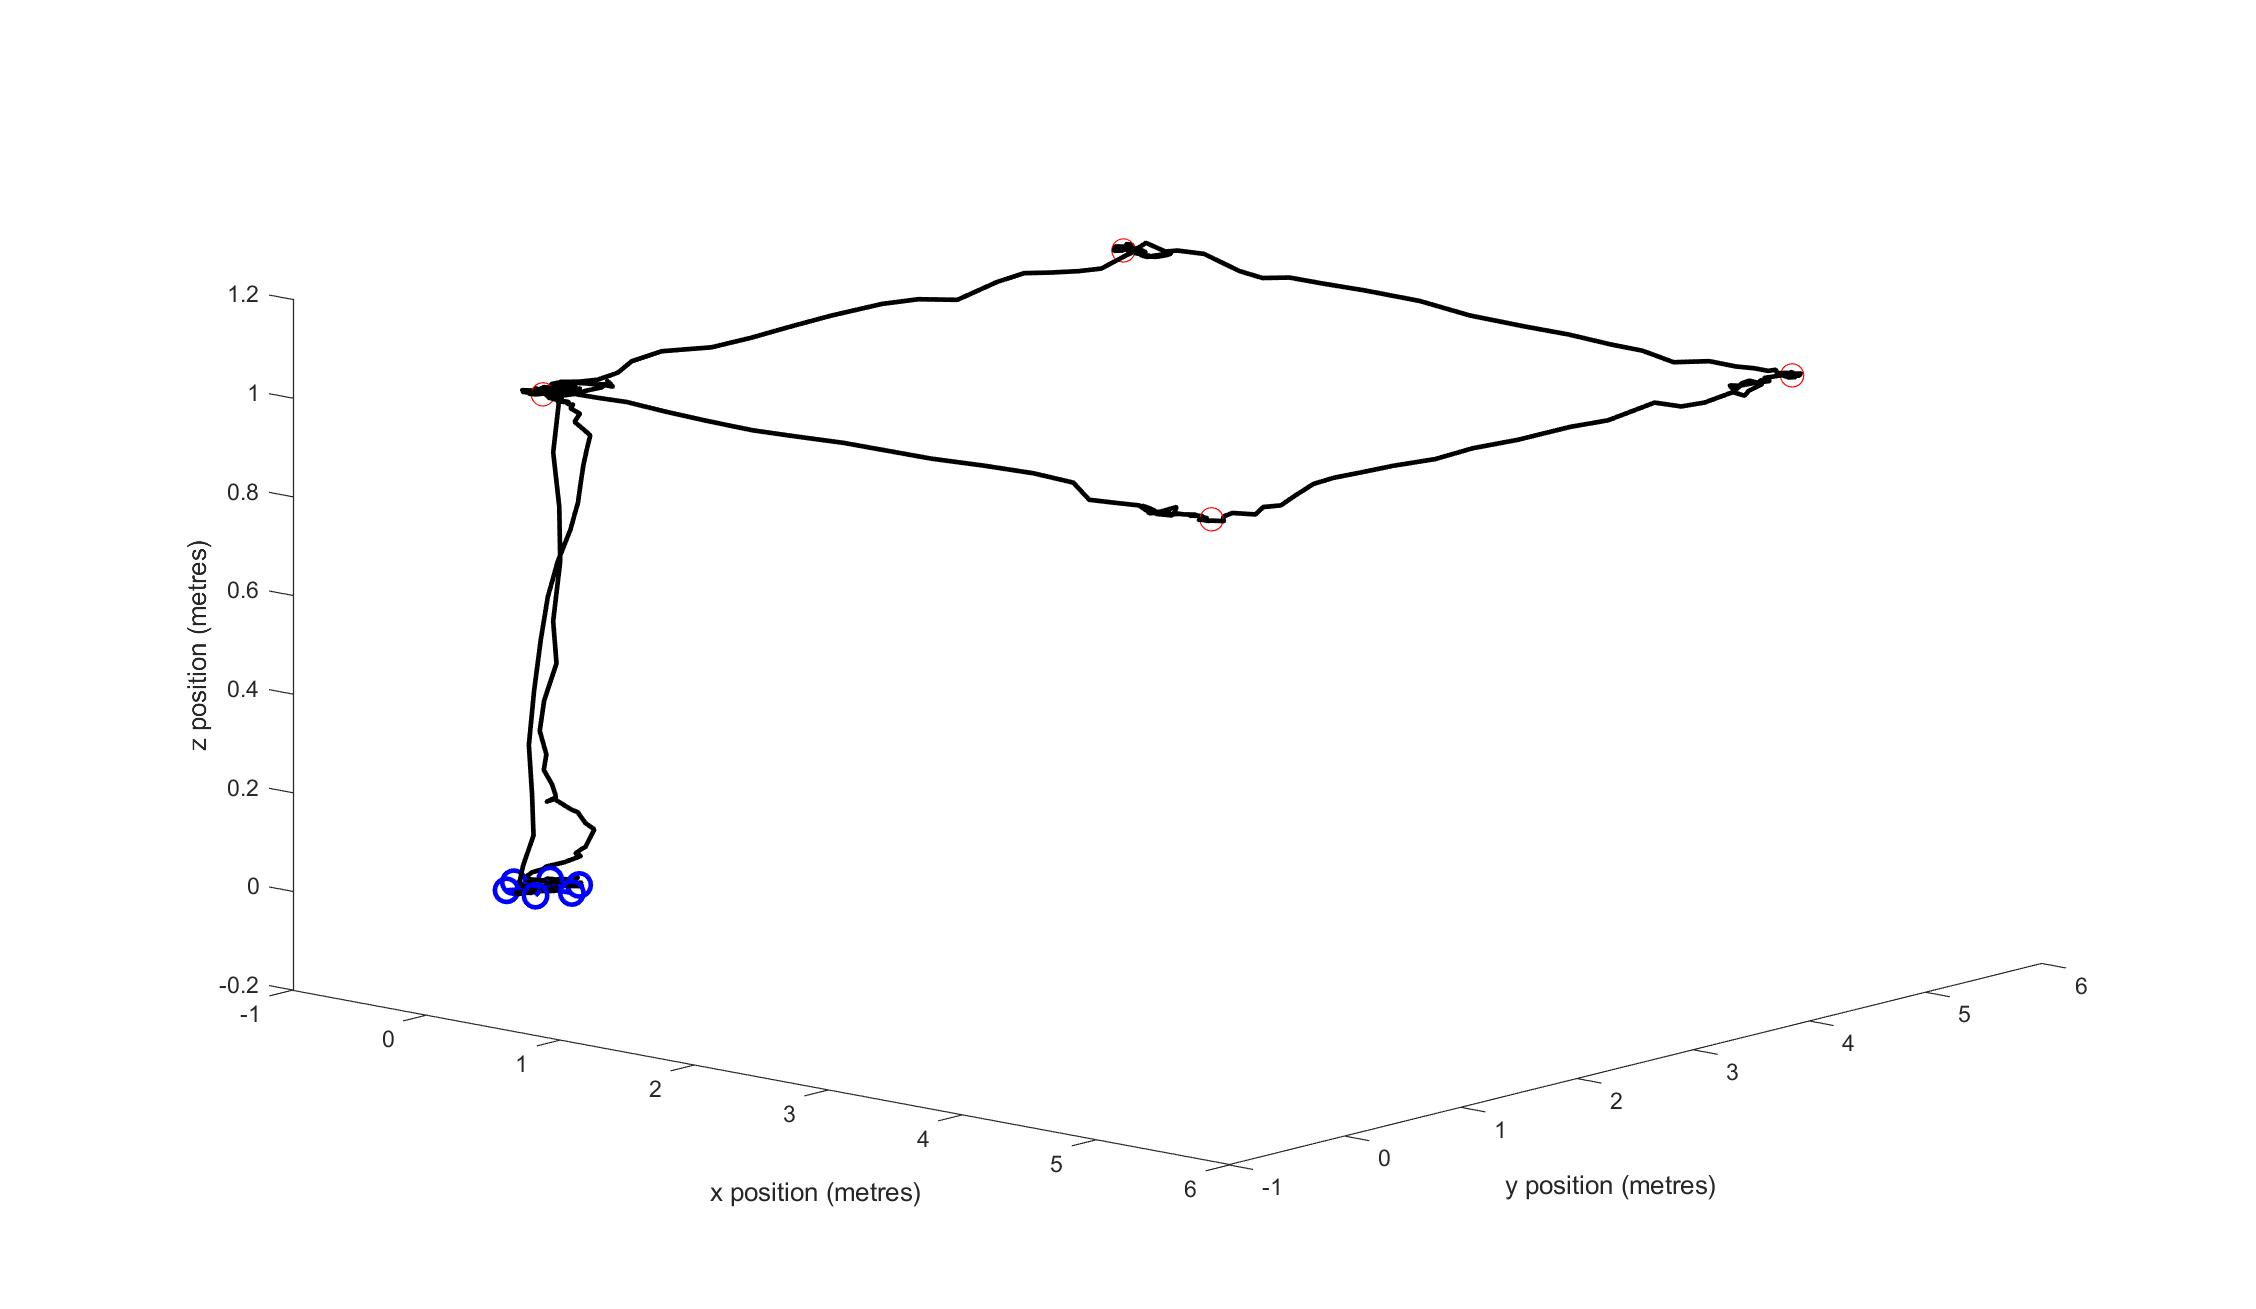
\includegraphics[width=\columnwidth]{/Saturation/WaypointsNoise.jpg}%
	\end{center}
	\caption{Final control system waypoint tracking with process noise.}%
	\label{fig:SatWayNoise}%
\end{figure}

\FloatBarrier
\section{Chapter Summary}
In this chapter, three control systems were developed and tested in simulation. The PID control system was effective at stabilising the aircraft around a hovering point, but had limitations due to not considering the nonlinearities of the system. The backstepping control system improved upon this by accounting for the nonlinearities, however this controller still depended on accurate values of the model parameters. The final controller implemented backstepping control with integral action and was effective in adjusting to errors in the given model parameters, however it was prone to actuator saturation with large step commands. The final addition to the control system implemented a sigmoid function in the position control laws to mitigate the effects of actuator saturation. These control systems were all developed with the assumption that all of the system states are available. The next section will address how the states are estimated using sensor data.



\clearpage



